\documentclass[11pt]{article}
\usepackage[a4paper, hmargin={2.8cm, 2.8cm}, vmargin={2.5cm, 2.5cm}]{geometry}
\usepackage{eso-pic} % \AddToShipoutPicture
\usepackage{graphicx} % \includegraphics
\usepackage{listings}
\usepackage{setspace}
\usepackage{cite}
\usepackage{stmaryrd}
\usepackage{fixltx2e}
\usepackage{amsmath}
\usepackage[utf8]{inputenc}
%\usepackage{fontspec}
\lstset{
  mathescape
  %moredelim=[is][\underbar]{_}{_}
}

\lstdefinelanguage{Futhark}{
  keywords={fun,fn,int,bool,char,if,then,else,let,in},
  keywordstyle=\color{blue!40!black}\bfseries,
  identifierstyle=\color{green!40!black},
}

\lstdefinelanguage{TAIL}{
  keywords={int,bool,char,if,let,in},
  keywordstyle=\color{blue!40!black}\bfseries,
  identifierstyle=\color{green!40!black},
}

\definecolor{Background}{rgb}{0.98,0.98,0.98}
\lstset{
    numbers=left,
    numberstyle=\footnotesize,
    numbersep=1em,
    xleftmargin=1em,
    framextopmargin=2em,
    framexbottommargin=2em,
    showspaces=false,
    showtabs=false,
    showstringspaces=false,
    frame=l,
    tabsize=4,
    % Basic
    basicstyle=\ttfamily\footnotesize\setstretch{1},
    backgroundcolor=\color{Background}
}

\author{
  \Large{Anna Sofie Kiehn (mvq686) \& Henriks Urms (mgs837)}\\
  \\ \textit{Supervisor: Martin Elsman}
  % \texttt{a.kiehn89@gmail.com} \\
  %\\ \texttt{a.kiehn89@gmail.com} \\ \\
  %\Large{Henriks Urms}
  %\\ \texttt{urmshenrik@gmail.com}
}

\title{
  \vspace{5cm}
  \Huge{Compiling TAIL to Futhark} \\
  \Large{- an adventure in compiling functional data-parallel constructs} \\
  \Large{$\;$} \\
  \Large{Bachelor's thesis} \\
  \Large{$\;$} \\
}

\setcounter{tocdepth}{2}

\begin{document}
%\renewcommand{\arraystretch}{1.2}

\newcommand{\evals}[1]{\llbracket #1 \rrbracket}

%% Change `ku-farve` to `nat-farve` to use SCIENCE's old colors or
%% `natbio-farve` to use SCIENCE's new colors and logo.
\AddToShipoutPicture*{\put(0,0){\includegraphics*[viewport=0 0 700 600]{include/natbio-farve}}}
\AddToShipoutPicture*{\put(0,602){\includegraphics*[viewport=0 600 700 1600]{include/natbio-farve}}}

%% Change `ku-en` to `nat-en` to use the `Faculty of Science` header
\AddToShipoutPicture*{\put(0,0){\includegraphics*{include/nat-en}}}

\clearpage\maketitle
\thispagestyle{empty}

\newpage

\abstract

We present an implementation independent scheme for the compiling of a subset of the intermidiate array language TAIL
 to the functional programming language Futhark, 
 preserving the data parallelism of the host language by using built-in data parallel functions in the target language to express the TAIL operations. We also present an implementation of the compilation scheme using this implementation to demonstrate the usefullness of compiling TAIL to Futhark by comparing the execution time of selected benchmarks on sequential backends to both languages, showing that the Futhark compiler optimises the execution time significantly. \\\\\\\\\\\\\\\\\\\\\\\\

\begin{center}
\textbf{Resumé}
\end{center}
Vi præsenterer et implementations uafhængigt oversættelses skema for en delmængde af det intermediære array sprog TAIL til det funktionelle sprog Futhark der bibeholder den data parallelisme der er i TAIL ved at bruge indbyggede data parallele funktioner i Futhark til at udtrykke TAIL operationerne i. Vi præsenterer også en implementation af skemaet og bruger denne implementation til at demonstrere anvendeligheden af at oversætte TAIL til Futhark ved at sammenligne udførselstiden af udvalgte benchmarks på sekventielle backends der viser at Futhark compilerens optimer udførselstiden betydeligt.

\newpage

\tableofcontents

\newpage

%%%%%%%%%%%%%%%%%%%%%%%%%%%%%%%%%%%%%%%%%%%%%
%%%%%%%%%%%%%%%%%%%%%%%%%%%%%%%%%%%%%%%%%%%%%
%%%%%%%%%%%  REPORT STARTS HERE  %%%%%%%%%%%%%%%%%%%%
%%%%%%%%%%%%%%%%%%%%%%%%%%%%%%%%%%%%%%%%%%%%%
%%%%%%%%%%%%%%%%%%%%%%%%%%%%%%%%%%%%%%%%%%%%%
\section{Introduction}
\label{intro}
In this paper we want to examine if it is possible, effectively to compile TAIL programs, produced by the APLTAIL compiler \cite{ElsmanDybdal:Array:2014}, into Futhark programs \cite{TroelsHenriksen} and thereby make use of the Futhark infrastructure for optimisation and the possibility for targeting parallel hardware.

In recent years, there has been a lot of focus on leveraging the power of parallel hardware. 
One approach has been to design programming languages with explicit data-parallel constructs that can be compiled 
into highly parallel code. One such language is Futhark \cite{TroelsHenriksen}. The aim of Futhark is to target parallel hardware such as 
GPUs while still being the target of more programmer-productivity oriented languages. The Futhark compiler 
performs several optimizations, such as fusion, which enhance the degree of 
parallelism \cite{T.Henriksen&C.Oancea} \cite{T2graph} \cite{Hybrid}.

APL (short for A Programming Language) \cite{APLbook} is an array language and includes various operations that are central to the language and are good candidates 
for parallel execution. Efforts in compiling APL to parallel backends already exist in the form of the language 
TAIL (Typed array intermediate language) and it’s compiler \cite{ElsmanDybdal:Array:2014}.
The TAIL compiler captures the parallelism inherent in APL source code and brings it to a much more manageable form.
In our work we provide a compiler from TAIL 
to Futhark thus bridging the gap between APL and Futhark.

The compilation between TAIL and Futhark is described in a compilation scheme that is the main contribution of this paper.
The compiler based on this scheme is called TAIL2Futhark. 
In Figure \ref{fig:compilers} is an overview of the main compilers mentioned in this project, it also show the code they produce.
The figure gives an overview of how the TAIL2Futhark compiler fits between the alredy existing APLTAIL compiler that compiles APL to TAIL code and the Futhark compiler that compiles Futhark to either sequential or parallel code C-code \cite{TroelsHenriksen}. 

The language Futhark is designed to target parallel architectures while at the same time acting 
as an intermediate language for more feature-rich languages.
By compiling APL to Futhark through TAIL the  Futhark compiler can be used to generate parallel code from APL once a parallel backend for Futhark is completed.

The background for designing TAIL was to create a typed intermediate language for the array programming language APL.
TAIL is still under development and so is the {\tt apltail} compiler which compiles a subset of APL into
TAIL \cite{ElsmanDybdal:Array:2014}.
APL is an older language created in the 1960's by Kenneth E. Iverson.
APL is an array programming language, its main type is the multi-dimensional array 
and most of the built-in functions in the language are array operators that work on this type. 
Most of its built-in functions or operators are represented by unicode symbols allowing for very concise code.
The APL language is dynamically typed. It supports first and second order functions and these functions work on arrays of any type. 
Even though it is an old language it is still used in the financial world 
where large code bases are still operational and actively developed \cite{ElsmanDybdal:Array:2014} \cite{Array:2015}.

One of the main point of interest in the compilation between TAIL and Futhark is compiling the four array operators 
of TAIL: {\tt each}, {\tt eachV}, 
 {\tt reduce} and {\tt zipWith} to Futhark source code that include the four second-order array combinators in Futhark:  
 {\tt map}, {\tt filter}, {\tt reduce} and {\tt scan} \cite{ElsmanDybdal:Array:2014}\cite{TroelsHenriksen}. 
However as the functionality of these functions is somewhat different the work lies in creating a mapping that retains the parallelism in the original code in the target language.
This can be seen in the example below which illustrate this difference. 
The APL code is given first. We do not describe APL in detail but the comments on each line should be explanation enough to understand what happens. 
%The reduce function in the
%TAIL language is mapped to a nested reduce function in the Futhark language.
%As the reshape function exists in both languages the Futhark version is \underline{underlined} for easier readability.
%
%$\text{reduce}$(+, [[1,2,3,4],[5,6,7,8]]))
%
%  =>
%
%$\underline{\text{reduce}}$(fn x => map(+,x),[[1,2,3,4],[5,6,7,8,]])

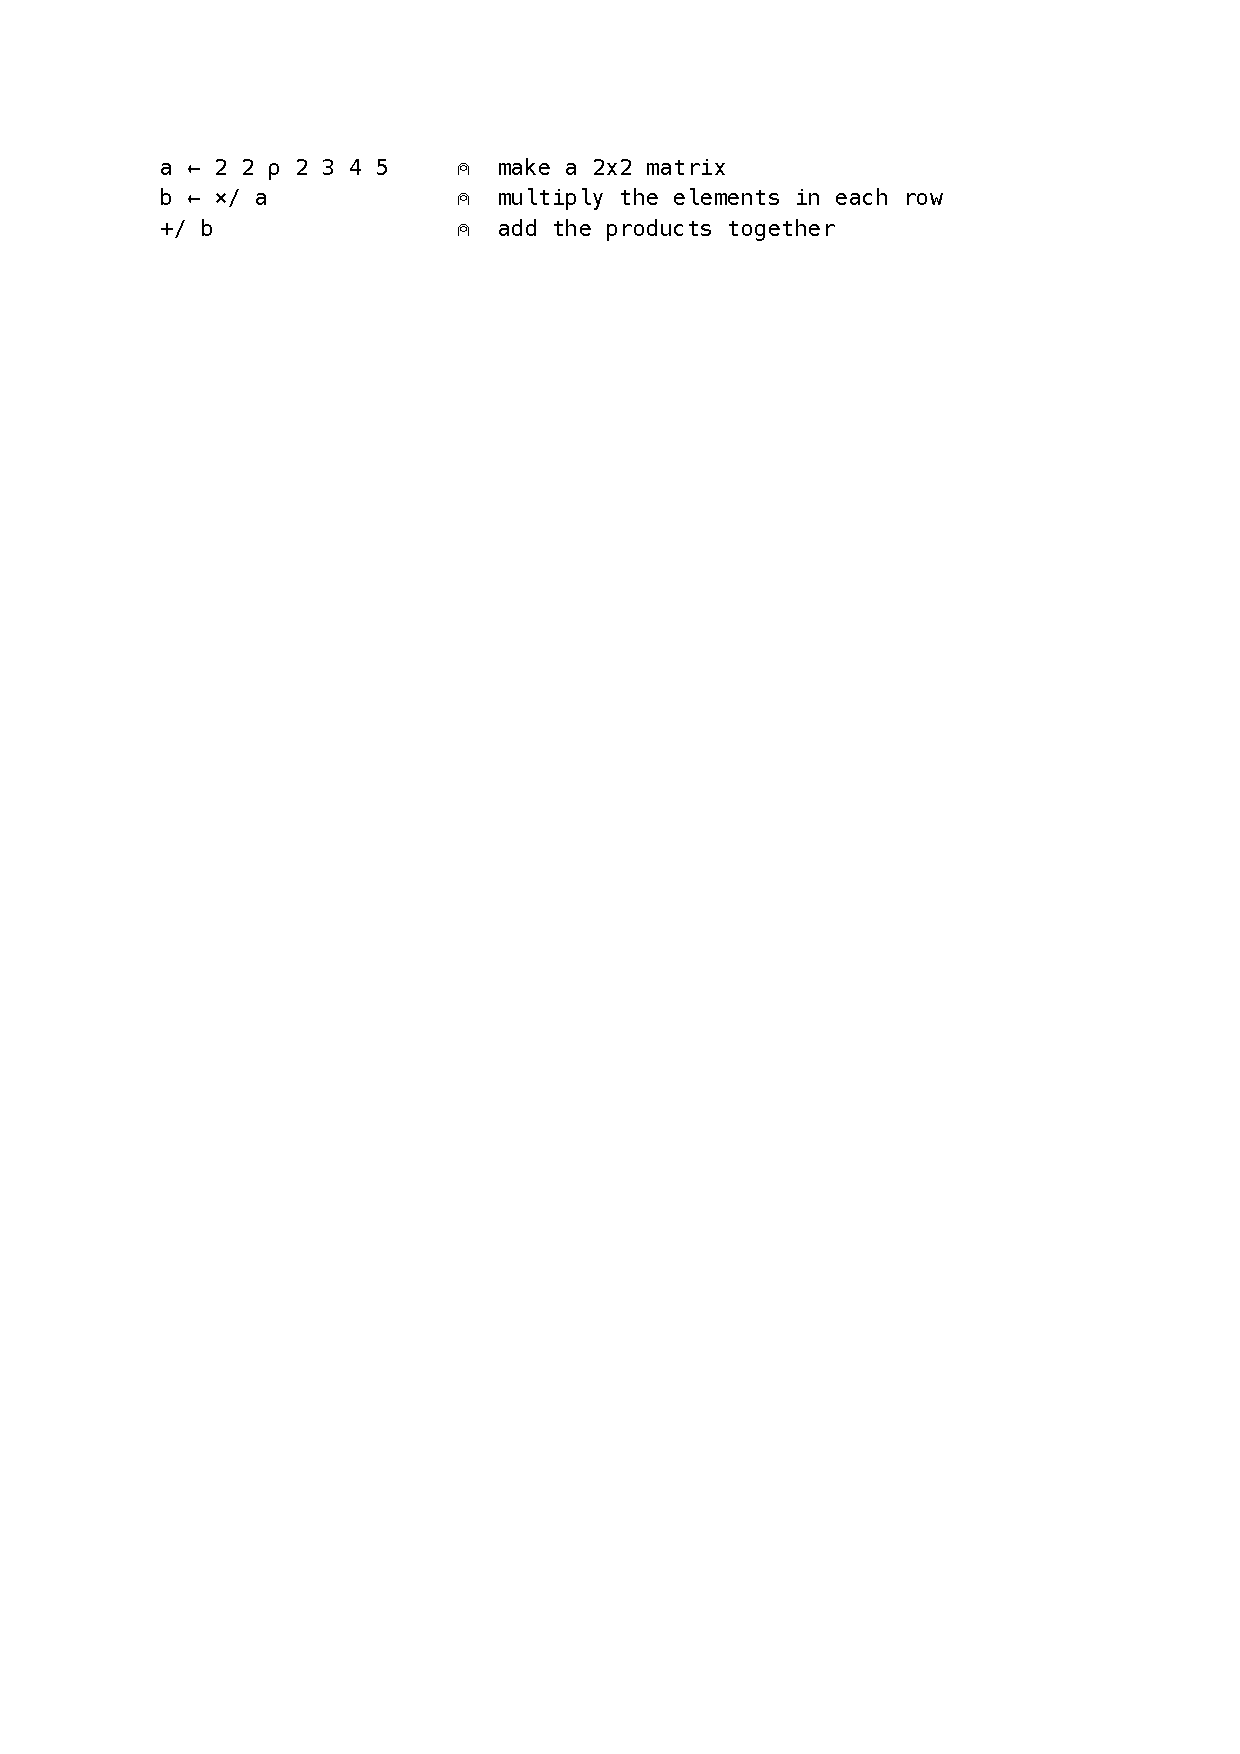
\includegraphics[scale=0.7,trim=6em 72em 10em 6em,clip=true]{reduce}

The APL code becomes the following TAIL code when using the APLTAIL compiler and now contains type information. The reason for the {\tt i2d} (int to double) operator is that the APLTAIL compiler only accept programs that returns doubles at the moment.


\begin{lstlisting}[numbers=none,frame=none,language=TAIL]
let v1:[int]2 = reshape{[int],[1,2]}([2,2],[2,3,4,5]) in
let v4:[int]1 = reduce{[int],[1]}(muli,1,v1) in
i2d(reduce{[int],[0]}(addi,0,v4))
\end{lstlisting}

This TAIL code is then compiled to Futhark code where the reduce function is mapped to a nested reduce function in the Futhark language. 

\begin{lstlisting}[numbers=none,frame=none,breaklines=true,language=Futhark]
fun real main() =
  let t_v1 = reshape((2,2),reshape1_int((2 * (2 * 1)),reshape(((size(0,[2,3,4,5]) * 1)),[2,3,4,5]))) in
  let t_v4 = map(fn int ([int] x) => reduce(*,1,x),t_v1) in
  toFloat(reduce(+,0,t_v4))
\end{lstlisting}

The nesting of the operator happens because the reduce function in APL and therefore TAIL works on the innermost dimention of the array but the reduce function in Futhark works on the outermost dimention of the array. In order to get the same functionality, namely reducing the content of the inner arrays the Futhark function have to be mapped unto them. This can be seen in the definition of the {\tt t\_v4} variable. 
The function {\tt reshape1\_int} is a library function that will be explained later. 

This paper contributes with a compilation scheme that are implementation independent, showing a replicable 
way of how to translate TAIL, to the functional language Futhark. Also 
this paper presents an implementation of the previous mentioned scheme in Haskell.
The efficiency of this implementation has been tested by comparing benchmark results on code generated by the C-backend to TAIL 
and the generated Futhark source code by using the C-backend to Futhark.
The project is open source and the source code can be found here:\\ https://github.com/henrikurms/tail2futhark.
Both Futhark and TAIL are ungoing research projects and are therefore subject to change bear in mind that the references cited may not be up to date (The versions used in this project was the versions available on github from Februar 2015 and until mid May 2015). For a up to date version of the languages and their compilers we refer to their recepctive github repositories (links for these repositories can be seen below): \\

TAIL: https://github.com/melsman/apltail

Futhark: https://github.com/HIPERFIT/futhark

The reader of this paper is assumed to have understanding of computer science consepts of the bachelor level and therefore general computer science terms (e.g. parser and compiler) will not be explained. 

% \section{Outline}
%The compilation scheme presented later in this section is written in a form of short hand notation to be able to have the entire compilation written in a short and very detailed was that is implem

\begin{figure}
\begin{center}
    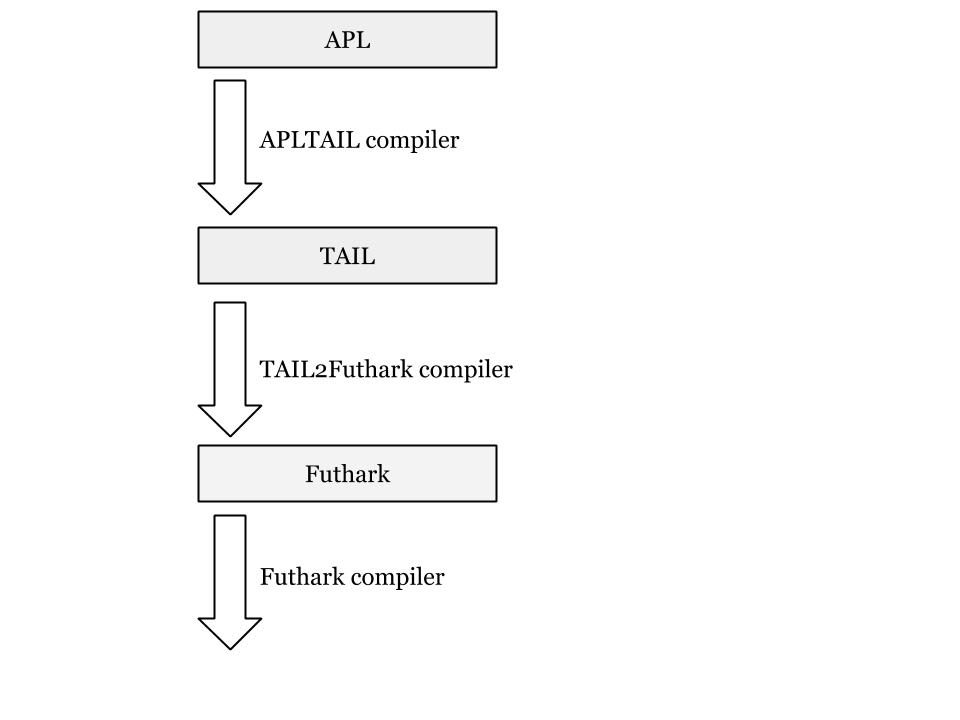
\includegraphics[width=4cm]{compilers.png}
    \caption{The three compilers used in this project and the code they produce }
    \label{fig:compilers}
\end{center}
\end{figure}

%The three main languages and compilers used in this project. The languages (APL, TAIL and Futhark) are shown as boxes. The compilers (APLTAIL, TAIL2Futhark and  Futhark) as arrows between the. In this project the creation of the TAIL2Futhark is shown.

\subsection{Scope}
In this project we create an implementation independent compilation scheme showing a compilation between TAIL and Futhark as well as a Haskell implementation of the compilation scheme, creating the TAIL2Futhark compiler. We also test the implementation of the compiler. 

We have used selected benchmarks that we will adabt to work with our project and present their results in section \ref{sec:benchmarks}. We will use benchmarks to see if the compiled Futhark code is more efficient than the original code. 

We will not do a detailed analysis of the results of the benchmarks or discuss the optimization that influence their running time.

We will not present an overview of APL but only reference to it. For a language reference pleace refer to \cite{APLbook} and \cite{APLDyalog}.

\subsection{Report outline}
The follwing sections of this paper is structured as follows. 
Section \ref{intro} includes the introductioin containing the scope and methods and tools used in this project. 
Section \ref{sec:tail} and Section \ref{sec:futhark} gives an introduction to the source and the target language. 
In Section \ref{sec:strategy} is a short presentation of the overall strategy for compiling TAIL to Futhark is given.
Section \ref{sec:scheme} describes the compilation scheme in detail. Secion \ref{sec:impl} is an overview of the Haskell implementation and tests. Section \ref{sec:benchmarks} describes the benchmarks used to messure the efficiency of the generated Futhark code by comparing it to the TAIL backend. Finaly Section \ref{sec:discussion} and Section \ref{sec:conclusion} is a discussion and conclusion of the results and contain ideas to possible future work. 

\subsection{Methods and tools}
\label{methods}
In this section we will describe and explain the reasoning behind the methods and tools we have used in the project. 

\subsubsection{Compilation scheme and the notation}
In this paper a compilation scheme done in a form of mathematical notation is presented. 
The reason for using a mathematical notation is to be able to express the compilation of the different componants of the compilation seperately and in a very detailed presice manner. We call the compilation of a specfic component a conversion rule. 
The notation should also be helpful in getting an overview of the entire main part of the compiler as well as creating a way of talking about specific conversions.
The notation is inspired by smimilar notation used in other projects \cite{TorbenMogensen}\cite{MartinElsmanNotation} to describe compilation schemes but is not built on a spefic standard as no such standard is known to us.
Instead we have invented our own notation.

The scheme gives a conceptual understanding of the compilation that are not cluttered by implementation details.
The scheme simply illustrates the concepts of the compilation an is implementation independent.
It should therefore be possible to use this model to create another implementation of the compiler.

Having the compilation scheme has also made the implementation easier because it helps to structure the implementation. 

\subsubsection{Library functions}
To keep the implementation scheme simple we have made a small library of functions which we present in section \ref{sec:library} 
We have coded the library functions in the compiler itself for various reasons
We would like the compiler to always output a valid (runnable) Futhark program given a valid TAIL input program, so we would like to
be able to include the library in the output when we run the compiler.
Furthermore since Futhark has no polymorphism we would like to be able to
generate functions with the same implementations but different types from a template.
That way we can be sure the different versions have the same implementation.
Finally because we expect Funthark to eventually feature polymorphism and a module system we would like the solution to not be too
extensive\cite{TroelsHenriksen}. 

\subsubsection{Choice of language for implementation}
The implementation described in this project is written in the functional programming language Haskell.
The language constructs in Haskell are smiliar to our mathematical notation and functional languages are good for developing compilers in general.\cite{TorbenMogensen}

\subsubsection{Other tools}
For building our project and managing external libraries we have used the cabal packaging system \cite{cabal}.
This is because cabal is the standard build architecture for Haskell and should make it easy to build our code.

We have created a Makefile for building our benchmarks. This made it much easier for us to rebuild the benchmarks and can also be used
as a reference of how to build them manually.

We have used the linux commandline tool {\tt time} for measuring the runtime of our benchmarks. 
It is not nessesary the best way but because of time constraints we have not looked for another solution.
One reason it is not ideal is because it also includes the time spend on reading data from files. We have however tried to create benchmarks where the execution of the computations overshadow any overhead created by this. In particular only one of our benchmarks read
data from files and the mesured difference between {\tt time} and a built-in timing function of the program only differed by 1 ms.

\subsubsection{Modifying an existing parser}
The parser we used for this project is created in a previous project that also worked with compiling TAIL to a parallel backend \cite{APLACC}. 
The latest version of the parser can be found in the github repository: https://github.com/mbudde/aplacc.
We did therefore not create the parser our selves,
instead we modified an existing parser where needed which enabled us to focus our work on the core of our project.

\section{TAIL}
\label{sec:tail}

In this section we present an overview on the language TAIL.

The syntax of types in TAIL can be seen below. Types are divided into base types ($\kappa$), shape types ($\rho$), types ($\tau$), and type schemes ($\sigma$).The letter $i$ denotes an integer scalar value and the letter $\alpha$, and the letter $\gamma$ denotes type variables and shape variables, respectively.
\begin{lstlisting}[numbers=none,frame=none]
$\kappa$ ::= int | double | bool | $\alpha$
$\rho$ ::=  $i$ | $\gamma$ | $\rho$ $+$ $\rho'$
$\tau$ ::= $[\kappa]^{\rho}$ | $\langle \kappa \rangle^\rho$ | S$_{\kappa}$($\rho$) | SV$_{\kappa}$($\rho$) | $\tau \rightarrow \tau'$
$\sigma$ ::= $\forall\vec{\alpha}\vec{\gamma}$.$\tau$
\end{lstlisting}
The type system of TAIL supports array types ($[\kappa]^{\rho}$) that keeps track of the rank of the array in its type.
The integer scalar in the array's shape type denotes the rank of the array and must be a non-negative integer.
The type system also supports vector types ($\langle \kappa \rangle^\rho$), which are used specifically to denote vectors of a specific length. For example, {\tt <int>8} denotes a vector of ints of known length 8. If a vector's length is not staticallly known, it can instead be expressed as an array of rank 1.
Scalar values that are statically known have a separate type (S$_{\kappa}$($\rho$)), that is integers, and booleans,
for which their value is contained in the type.
In addition, there also exists single-element integer, double, and boolean vector types (SV$_{\kappa}$($\rho$)) for singleton vectors where the element is statically known.
Finally there exists function types ($\tau \rightarrow \tau$').

%The types schemes ($\sigma$) are expressed through substitution...
The type system makes use of substitution in order to express instances of type schemes ($\sigma$).
A type substitution ($S_t$) maps type variables to base types and shape substitution ($S_s$) maps shape variables to shape types.
A general substitution ($S$) is a pair ($S_t$,$S_s$) of a type substitution and a shape substitution.
Using the substitution $S$ on an object $B$ means applying both $S_t$ and $S_s$ on objects in $B$.
A type $\tau'$ is an instance of a type scheme $\sigma$ = $\forall\vec{\alpha}\vec{\gamma}$.$\tau$ (written $\sigma$ $\geq$ $\tau'$) if a substitution $S$ exists such that $S(\tau)$ = $\tau'$. All type schemes are assumed closed.

The syntax of operators and expressions is given below. The letter $v$ is used to denote values and the letter $x$ is used to denote program variables. 
\begin{lstlisting}[numbers=none,frame=none]
$op$ ::= addi | subi | multi | mini | maxi | addd | subd | 
       muld | mind | maxd | andb | orb | xorb |  nanb | 
       norb | notb | lti | ltei | gti | gtei | eqi | neqi |
       ltd | lted | gtd | gted | eqd | neqd | iota | each |
       reduce | i2d | b2i | reshape0 | reshape | rotate |
       transp | transp2 | zipWith | shape | take | drop |
       first | cat | cons | snoc | shapeV | catV | consV | 
       snocV | iotaV | rotateV | takeV | dropV | firstV 

$e$ ::= $v$ 
    | $x$ 
    | $[\vec{e}]$ 
    | $e$ $e'$ 
    | let $x$ = $e_1$ in $e_2$ 
    | $op(\vec{e})$

$v$ ::= $[\vec{a}]^{\delta}$
    | $\lambda x.e$
\end{lstlisting}
A TAIL program always consists of a single expression. An expression can then be a value, a variable, 
a list of expressions, a let expression or an operator. Each TAIL operator has a unique type scheme.

One of the operators with a simple type scheme is the binary operator maxi that takes two arguments $a$ and $b$ and evaluates to the argument with the highest value. Its type scheme is as follows:
\begin{lstlisting}[numbers=none,frame=none]
maxi : int $\rightarrow$ int $\rightarrow$ int
\end{lstlisting}

Other operators have more complex type schemes. Examples of those are the parallel operators. 
There are four parallel operators in the subset of TAIL that we consider, namely {\tt each}, {\tt eachV}, {\tt reduce} and {\tt zipWith}.
The functions {\tt each} and {\tt eachV} are known in many languages as map.
The type scheme for the function {\tt each} is:
\begin{lstlisting}[numbers=none,frame=none]
each : $\forall\alpha\beta\gamma.(\alpha \rightarrow \beta)\rightarrow [\alpha]^{\gamma} \rightarrow [\beta]^{\gamma}$
\end{lstlisting}
Given a function $f$ and an array $a$, the application {\tt each(f,a)} evaluates to an array where $f$ is applied to each element of $a$ given the value $[f(a_1),..,f(a_n)]$.
If the rank of the array is greater than 1 the {\tt each} function works as a map on the fattened representation of the array,
that is, the function is applied on the inner most dimension of the array, or seen in another way, on each basic value.

The {\tt eachV} function is a special case of {\tt each} and is used on vector types.

The function {\tt reduce} works similaly to fold known from functional languages. The type scheme for {\tt reduce} is:
\begin{lstlisting}[numbers=none,frame=none]
reduce : $\forall\alpha\gamma.(\alpha \rightarrow \alpha \rightarrow \alpha)\rightarrow \alpha \rightarrow [\alpha]^{1 +\gamma} \rightarrow [\alpha]^{\gamma}$
\end{lstlisting}
The function takes as arguments an associative binary operator $op$ (for instance $+$), a neutral element $n$, (for instance 0) and an array $a$.
The function application evaluates to the reduction of the elements using the operator.
An array of rank $\gamma+1$ is reduced to an array of rank $\gamma$ along the inner-most dimension.
Unlike fold, reduce makes no guarantees as to the order of application of the operator, therefore the operator has to be associative and the element has to be neutral, this is of course necessary for parallel execution.

The {\tt zipWith} function's type scheme is given as follows: 
\begin{lstlisting}[numbers=none,frame=none]
zipWith  : $\forall\alpha_{1}\alpha_{2}\beta\gamma.(\alpha_1 \rightarrow \alpha_2 \rightarrow \beta)\rightarrow [\alpha_1]^{\gamma} \rightarrow [\alpha_2]^{\gamma} \rightarrow [\beta]^{\gamma}$
\end{lstlisting}
Given a function $f$ that works on a pair $(x,y)$ and two arrays $a$ and $b$, {\tt zipWith(f,a,b)}  evaluates to an array where the i'th element is $f$ applied to the pair $(a_i,b_i)$ 
Like the other three operators, it works on the inner-most dimension of the array\cite{ElsmanDybdal:Array:2014}.

There are other important operators besides the parallel ones. One of them is the operator {\tt reshape($a_1$,$a_2$)}.
Given two arrays it reshapes the flattened representation of the second array $a_2$ to the shape given by the first array so $([2,3],[1,2,3,4,5,6])$ evaluates to $[[1,2,3],[4,5,6]]$. 
If $a_2$ is too long the elements not needed are dropped. That is, $reshape([2,3],[1,2,3,4,5,6,7,8])$ would evaluate to the same as the first example.
If $a_2$ is shorter than needed the elements of $a_2$ are repeated. That is $reshape([2,3],[1,2,3])$ evaluates to $[[1,2,3],[1,2,3]]$. Note that this is not how arrays are represented in TAIL. Instead of using nested brackets to represent the dimentions, arrays in TAIL are represented with a shape (i.e. $[1,2,3,4,5,6]^{[2,3]}$). However, using this representation can make what happens less obvius so we use the nested brackets representation insted. 

Other important operator expressions are {\tt take($i$,$a$)} and {\tt drop($i$,$a$)}.
They return an array containing the 1st to $i$'th element of $a$,
and the array containing the $i$'th to n'th element of $a$, respectively.
If the array is multi-dimensional, the operators work on the outermost dimesion of the array. That is $take(2,[[1,2],[3,4],[5,6]])$ evaluates to $[[1,2],[3,4]]$.
If the array contains too few elements the array is padded with zeros,
whereas the {\tt drop} operator returns the empty array in the case that more elements are dropped that than $a$ contains. 

The operator {\tt snoc(a,e)} takes two arrays $a$ and $e$ and returns an array where the i'th element of $e$ is appended onto the end of the i'th row of $a$.
If there are too few elements in $e$ an error occurs,
except if there is only one element in $e$ in which case the operator evaluates to an array where the one element from $e$
is appended onto each row of $a$.

The operator {\tt cons(e,a)} has very similar semantics as the {\tt snoc} operator.
The only difference is that it appends the contents of $e$ not on the end but at the beginning of each row.

The operator {\tt cat($a_1$,$a_2$)} takes two arrays that have to have the same outer dimension and returns an array where the i'th element (for instance a row if the array is two-dimensional) of $a_2$ is appended onto the end of the i'th element of $a_1$.

The {\tt transp} operator takes an array and returns the transposed array. For instance,
 $transp([[1,2,3],[4,5,6]])$ evaluates to $[[1,4],[2,5],[3,6]]$.
If the array is multi-dimensional (i.e. a three-dimensional array with the shape $2\times3\times4$) the function returns an array with the shape $4\times3\times2$.

TAIL was designed with the purpose of targeting parallel architectures such as GPUs and allows parallel programs to be
expressed in a highly abstract manner.
The TAIL compiler can also efficiently compile TAIL code into sequential code in a C-like language.
The subset of APL operators that TAIL support are shown earlier in this section.
The TAIL compiler infers types for the values in the APL program and can annotate bindings with
instance declarations. An instance list provides the base type and rank of the array. Or in
the case of vectors the size of the vector.
The language TAIL is statically typed and supports polymorphism. 
Most of the operators in TAIL are very general that is, they are polymorphic with respect to array ranks and base types.
Although for some operations a specific type is needed.
An example is the {\tt take} function. It takes as argument a number (of type int) and an array of type $[\alpha]^\gamma$.

TAIL's type system takes the dynamic types of APL and transforms it to a more manageable form adding explicit type
information to the constructs.
Another benefit of the expressiveness of TAILs type system is that it allows the (TAIL) compiler to express some operators which
are primitive in APL using simpler operators, one such operator is that of the inner product \cite{ElsmanDybdal:Array:2014}. 

The aplacc parser for TAIL represents the TAIL expressions in the abstract syntax tree as variables, constants, infinity, the negative representation of 
the expression, let expressions, operators and lambda expressions. 

% THIS IS HOW THE COMPILER IMPLEMENTS EXPRESSIONS
%\begin{lstlisting}[numbers=none,frame=none]
%e ::= x | i | d | c | inf | -e | let x:$t$ = e$_1$ in e$_2$ |
%      op[e$_1$,...,e$_n$] | fn x:$t$ e | [e$_1$,...,e$_n$]
%\end{lstlisting}

Generally it is not possible to define higher-order lambda expressions in TAIL, however higher-order operators
may use currying of lambda expressions to express multi-argument functional arguments.
This means lambda expressions that evaluate to lambda expressions can occur as arguments in higher-order operator
applications and nowhere else.

% In APL indexing are done with 1-indexing but it is possible to change the indexing to 0-indexing on the fly. 

%So far TAIL only support a subset of the APL functions and operators. 

\section{Futhark}
\label{sec:futhark}

In this section we give a short introduction to the Futhark language. We will only cover the parts necessary to understand
the reasoning behind our compilation approach. For the full language reference please refer to \cite{TroelsHenriksen}.

The syntax of Futhark types can be seen below.
\begin{lstlisting}[numbers=none,frame=none]
$t$   $::=$   int          (Integers)
    | real         (Float)
    | bool         (Booleans)
    | char         (Characters)
    | {$t_1$,...,$t_n$}      (Tuples)
    | [t]          (Arrays)
    | *[t]         (Unique arrays)
\end{lstlisting}
The types in Futhark consist of: integers, floating points, booleans, and chars, tuples (\lstinline |{t$_1$,...,t$_n$}|), arrays ({\tt [t]}), and unique arrays ({\tt *[t]}).
Tuple types are written as a comma separated list of types or values surrounded by braces.
For example \lstinline|{int,bool}| represents pairs of integers and booleans.
Unlike TAIL, Futhark allows nesting of arrays and indeed nested arrays are how multi-dimensional arrays are expressed in Futhark.
Array types are denoted by the elements (base) type enclosed by brackets.
The layer of brackets indicates the dimensionality of the array type.
For instance {\tt [int]} is a one-dimensional array of integers, and {\tt [[[bool]]]} is a tree-dimensional array of booleans.
Arrays must be regular, that is, all arrays in an array must have the same number of elements.

The Futhark language is statically typed but does not use type inference.
Also, the type system of Futhark is not able to express polymorphism, which means that it is not possible to make polymorphic functions in Futhark.
The exception to this rule is that a lot of the built-in functions can be used on multiple types.

The syntax of Futhark expressions is show below as follows:
\begin{lstlisting}[numbers=none,frame=none]
$k$ ::= $n$				(Integer)
    | $d$				(Decimal number)
    | $b$				(Boolean) 		
    | $c$ 				(Character)
    | {$v_1$,...,$v_n$} 		(Tuble)
    | [v$_1$,...,$v_n$] 		(Array)
\end{lstlisting}

\begin{lstlisting}[numbers=none,frame=none]
$e$ ::=  $k$								(Constant)
    | $v$ 								(Variable)
    | {$e_1,...,e_n$} 							(Tuble expression)
    | [$e_1,...,e_n$] 							(Array expression)
    | $e_1$ $\odot$ $e_2$ 							(Binary operator)
    | $-e$ 								(Prefic minus)
    | !$e$ 							(Logical negation)
    | if $e_1$ then $e_2$ else $e_3$ 				(Branching)
    | $v$[$e_1,...,e_n$] 							(Indexing)
    | $v$($e_1,...,e_n$) 							(Function call)
    | let $p$ = $e_1$ in $e_2$					(Pattern binding)
    | zip($e_1,...,e_n$) 						(Zipping)
    | unzip($e$)						(Unzipping)
    | iota($e$) 						(Range)
    | replicate($e_n, e_v$) 					(Replication)
    | size($i$,$e$) 						(Array length)
    | reshape(($e_1,...,e_n$),e)					(Array reshape)
    | transpose($e$)					(Transposition)
    | split($e_1,e_2$)						(Split $e_2$ at index $e_1$)
    | concat($e_1,e_2$)						(Concationation)
    | let $v_1$ = $v_2$ with					(In-place update)
             [$e_1,...,e_n$] <- $e_v$ in $e_b$
    | loop ($p$ = $e_1$) = for $v$ < $e_2$ do		(Loop)
             $e_3$ in $e_4$
\end{lstlisting}
\begin{lstlisting}[numbers=none,frame=none]
$p$ ::= $id$ 
    | {$p_1$,...,$p_n$}
\end{lstlisting}

\begin{lstlisting}[numbers=none,frame=none]
$fun$ ::=  fun t v(t$_1$ v$_1$,...t$_n$ v$_n$) = $e$
\end{lstlisting}

\begin{lstlisting}[numbers=none,frame=none]
$prog$ ::= $\epsilon$ | $fun$ $prog$
\end{lstlisting}

\begin{lstlisting}[numbers=none,frame=none]
$l$ ::=  fn $t$ ($t_1$ $v_1,..., t_n$ $v_n$) => $e$			(Anonymus function)
    | $id$ ($e_1,...,e_n$)					   (Curried function)
    | op $\odot$ ($e_1,..., e_n$)			   	   (Curried operator)
\end{lstlisting}

\begin{lstlisting}[numbers=none,frame=none]
$e$ ::=  map($l$, $e$)					
    | filter($l$, $e$)
    | reduce($l$, $x$, $e$)
    | scan($l$, $x$, $e$)
\end{lstlisting}




Note that the syntactical construct denoted by $l$ can only occur in {\tt map}, {\tt filter}, {\tt reduce} and {\tt scan}.
The functions {\tt map }, {\tt filter }, {\tt reduce } and {\tt scan } are second-order array combinators, or SOACs for short.

The SOACs operate on arrays with first-order functions given as arguments.
Functional arguments used can be function names of first-order functions (either user-defined or built-in), 
binary operators, or lambda expressions.
Futhermore in a SOAC expression operators and functions can be curried. Lambda expressions require explicit type annotations for
the return type and argument types, and argument bindings follow the normal shadowing rules.

We do not target the SOACs {\tt filter} and {\tt scan} in our compilation, and we will therefore not discuss them in detail here.
The SOACs can be used on arrays of any type even though it cannot be expressed by Futhark types.
For clarity we give the type for each SOAC that it would have had in a polymorphic language.
Below we shortly discuss {\tt map} and {\tt reduce}.

The function {\tt map} has the following type: 
\begin{lstlisting}[numbers=none,frame=none]
map : $\forall\alpha\beta.(\alpha \rightarrow \beta) \rightarrow [\alpha] \rightarrow [\beta]$
\end{lstlisting}
The function {\tt map($l$,$a$)} takes a function $l$ and an array $a$ and evaluates to the array consisting of $l$ applied to each element of $a$.
In contrast to TAIL, if the array is multi-dimensional the function is applied to the outer most dimension.
This means that if the function $l$ is mapped into a 2-dimensional array the function would be applied to an array not the elements
of the array. This makes sense considering that Futhark represents multi-dimensional arrays using nested arrays.

The type of the function {\tt reduce} is: 
\begin{lstlisting}[numbers=none,frame=none]
reduce : $\forall\alpha.(\alpha \rightarrow \alpha \rightarrow \alpha)\rightarrow \alpha \rightarrow [\alpha] \rightarrow \alpha$
\end{lstlisting}
Given a binary operator/function $l$, the neutral element $e$ of $l$ and an array $a$,
{\tt reduce } evaluates to the result of applying $l$ to combine all the elements of $a$, that is,
\begin{lstlisting}[numbers=none,frame=none]
$e \odot a[0] \odot \ldots \odot a[n]$ where $x \odot y = l (x,y)$
\end{lstlisting}
Like {\tt map}, {\tt reduce} applies the function on the outer-most dimension of the array \cite{TroelsHenriksen}.

The first-order segment of Futhark has many of the typical language features like constants, variables, many of the usual binary operators, branching, array indexing and some additional features like in-place updates and looping which we do not use.

Futhark features array zipping with the built-in {\tt zip} which produces an array of pairs from a pair of arrays.
The resulting arrays can then be mapped over with binary operators such as +.

The {\tt iota} function given an integer $n$ produces an array with integer values ranging from 0 to $n-1$.
The {\tt replicate} function given an integer $n$ and an array $a$ returns an array consisting of $n$ copies of $a$.
The {\tt size} primitive will given a positive integer $i$ and an array $a$ return the i'th dimension, or put in another way
the length of the arrays nested with depth $i$ in $a$. Remember that these arrays will all have the same length.
The {\tt reshape} function takes a number of dimensions $(dim_1,..., dim_n)$ and an array $a$ and returns an array where the elements of $a$ is reshaped into the shape specified by the list of dimensions.
The number of elements in $a$ must be equal to the product of the dimensions i.e. $elements$ $of$ $a$ $=$ $dim_1 * ... * dim_n$.

The function {\tt transpose} take an array $a$ and return the transposed $a$.
Transposing a three-dimensional array with dimensions $2 \times 3 \times 4$ is not like in TAIL an array with dimensions $4\times3\times2$ but instead an array with dimensions $3\times4\times2$.

The function {\tt split} given an integer $n$ and an array $a$ partitions $a$ into two arrays $a[0,..,n]$ and $a[n+1,...]$ and returns them as a tuple. 
The function {\tt concat} takes two arrays and concatenates them by concatenating the row/elements of one array with another. The shape of the two arrays have to be the same except in the first dimension. 

The undocumented {\tt rearrange} function takes as arguments a comma separated list of dimensions (surrounded in parentheses) and an array. It then rearranges the shape of the array to the by the list specified.

The aim of Futhark is to be an attractive choice for expressing complex parallel programs.
This goal is pursued by featuring high expressive power without
losing the ability to do aggressive optimization and managing parallelism.
This is a challenge because higher expressive power means optimizations become more difficult. 
However Futhark does support nested parallelism as this is a feature many programs 
depend upon even though it does make optimization more difficult \cite{TroelsHenriksen}.

% funktioner bliver inlinet

% funktioner skla definere returtype og type på alle argumenter

%Does not support polymorfism in types

\section{The compilation strategy}
\label{sec:strategy}
Where possible, TAIL primitives have been mapped directly to their corresponding versions in the Futhark language.
Where direct translation is not possible the approach has been to use exisiting operations as much
as possible and generate code to bridge the gap.

%map -> map
% use map
% don't use loops
% no optimizations (rely of futhark optmizations)
% library functions to simplify compilation

%The first case is for example seen in the compilation of let-expressions and many of the basic scalar operators (e.g. plus).
%The second case is seen in for example the compilation of the iota operator.

The general strategy for compiling TAIL expressions was to aim for the simplest conversion and use as much as possible 
the built-in functions of Futhark to make it easy for the Futhark compiler to optimise away the overhead that the compilation from TAIL to Futhark may have created.
This means we have not directly focused on optimization in the compilation as it was futhermore not in the scope of this project.
Still we have tried as much as possible to not introduce any unecessary inefficiencies.
 %(et eller andet med det overhead eller sådan noget som vi potentielt kan have skabt kva at vi stort set ikke har tænkt på hvad der er optimalt.)

In the cases where it was not posible to use built-in Futhark functions library functions was created instead. 
%There are several reasons for making libary functions. One was to keep our compilation scheme simple.
%By having a small library of Furhark functions which is inlined in each compiled program we... % ja hvad får vi egentlig ud af det??? :)

Many of the monomorphic first-order functions of TAIL are mapped directly to a library function of the same name. This also allows us to use the same mapping when the functions occur as arguments in SOAC applications.

% Er der flere fordele ved biblioteksfunktionerne??
% Hvad er det negative ved biblioteksfuntionerne
% Hvad var alternativet 

\section{Library functions}
\label{sec:library}
In this section explain some of the nontrivial library functions we have defined and discuss their usefulness. The rest of the  library functions can be found in the end of this section. 

\subsection{The take1, drop1 and reshape1 functions}
The {\tt take1}, {\tt drop1} and {\tt reshape1} functions implement the TAIL operators {\tt take}, {\tt drop} and {\tt reshape} in the one-dimensional case. In Section \ref{sec:scheme}, we see how they can be used to implement the multi-dimensional cases. It is advantageous to use a library function for only the one-dimensional case as we would otherwise need a separate library function for each 
rank and basic type combination which we then needed to call since Futhark only allows declaration of monomorphic functions \cite{TroelsHenriksen}.
We have implemeted the functions (take1, drop1, and reduce1) as templates written in Haskell. 
A template is a function that given a type returns Futhark code for that function with the given type.
We have done this so we can use the same template for making all four functions (one for each base type) and can thereby be sure to have the same function code for each type and make maintaning the functions easier. 

\subsubsection{The take1 functions}
The {\tt take1} functions is defined as follow: 
\begin{lstlisting}[language=Futhark]
fun [int] take1_int(int l,[int] x) =
  if (0 <= l)
  then if (l <= size(0,x))
       then let {v1,_} = split((l),x) in v1
       else concat(x,replicate((l - size(0,x)),0))
  else if (0 <= (l + size(0,x)))
       then let {_,v2} = split(((l + size(0,x))),x) in v2
       else concat(replicate((l - size(0,x)),0),x)
\end{lstlisting}
Note that this is the {\tt int} version. The template is as menstioned used to make a boolean, char, and float version as well but we have chosen only to show one for space reasoons. 

The function first checks if it should perform a positive of negative take and then checks whether it should split so it can return
part of the argument or pad the argument with zeros based on whether the take size was smaller or bigger than the array.

%TODO what details are we missing?
%TODO discuss how it knows what to pad with
\subsubsection{The drop1 functions}
The {\tt drop1} functions is defined as follows: 
\begin{lstlisting}[language=Futhark]
fun [int] drop1_int(int l,[int] x) =
  if (size(0,x) <= if (l <= 0) then -l else l)
  then empty(int)
  else if (l <= 0)
       then let {v1,_} = split(((l + size(0,x))),x) in v1
       else let {_,v2} = split((l),x) in v2
\end{lstlisting}
Again we show only the int version. 

\subsubsection{The reshape1 functions}
The {\tt reshape1} function's int version can be seen below.

To adjust the array we first make sure it is long enough by extending it using the function replicate and then
truncate it to the correct length with split.

\begin{lstlisting}[language=Futhark]
fun [int] reshape1_int(int l,[int] x) =
  let roundUp = ((l + (size(0,x) - 1)) / size(0,x)) in
  let extend = reshape(((size(0,x) * roundUp)),replicate(roundUp,x)) in
  let {v1,_} = split((l),extend) in v1
\end{lstlisting}

When we replicate an array in Futhark the rank of the array increases by one so we have to reshape the array back to rank 1 before we split it.
The number of times we should replicate the array is the target size divided by the array size rounded up.
This is computed in the variable roundUp, we add denominator plus one to the enumerator to round up as normal integer division round down.

%Nevertheless we inline the flattening and reshaping code so we only need reshape functions written in Futhark
%for the one dimensional cases. If we wanted to simply call a function instead we would need a separate library function for each
%rank and basic type combination which we needed to call reshape on since Futhark only allows declaration of monomorphic functions \cite{TroelsHenriksen}.

\subsection{Bool equality}

Futhark has no bool equality so we implemented our own:

\begin{lstlisting}[language=Futhark]
fun bool eqb(bool x,bool y) =
  (!((x || y)) || (x && y))
\end{lstlisting}

Two booleans are equal if they both are true or none of them are true.

\subsection{Xor} Likewise there is no logical xor operation so we included it in the library:

\begin{lstlisting}[language=Futhark]
fun bool xorb(bool x,bool y) =
  (!((x && y)) && (x || y))
\end{lstlisting}

The Xor of two booleans is true if one but not both of them are true.

\subsection{All other library functions}
The rest of the library functions are implemented very straight forward and are therefore only mentioned as a list here:

\begin{lstlisting}[numbers=none,frame=none]
boolToInt,negi,negd,absi,absd,mini,mind,signd,signi,maxi,maxd,
nandb,norb,neqi,neqd,resi
\end{lstlisting}
The implementation of these functions can be found the compiler source code in Appendix \ref{app:impl}

\section{The compilation scheme}
\label{sec:scheme}

There main contribution with this paper as mentioned earlier is the compilation scheme presented in this section.
It shows a set of conversion rules of a subset of TAIL's syntax to Futhark source code.
The notation is explained and the compilation of some of the nontrivial operators or expressions of TAIL is described in detail. 

The main part of the compilation scheme that contains the expressions can be seen in Figure
\ref{fig:compilationscheme}.
In Figure \ref{fig:lambdas} is the conversion rules for lambda expressions.
In Figure \ref{fig:funs} are the functions that are compiled directly to a corresponding function in Futhark and in Figure \ref{fig:binops} are the compilation of the binary operators. Note that the schemes in the above mentioned figures are all mutually recursive. 

When $e$ is some TAIL expression, and $e'$ is some Futhark expression we specify the translation as rules of the form $\evals{e} = e'$. The rules are syntax-directed in the sense that they follow the structure of $e$, recursively. 

% Presentation of the compilation scheme
% Explain the reson for making the scheme
%% Implementation independent overview of the compilation
%% A way to easy create an overview thereby limiting the chances that we missed something
%% Easy for others to use 
%% way to get the ide down on paper
% Explain the notation/ who to read the scheme
%% how is it possible to destinct between futhark and tail functions/expressions 
%% how is the types represented og hvad betydning har de
% Explain the general idea behind the compilation
%% try to use futhark functions whenever posible.
%% inlined library functions to deal with cases where no futhark function existed or polymorphism was required
%%% explain WHY we chose libraryfunctions and what the alternative was. 
% Walkthrough of some of the more interesting compilations. Explain WHY we did what we did. 
%\newgeometry{top=15pt,left=30pt,bottom=70pt}
%\begin{flushleft}

\begin{figure}
\begin{tabular}{@{}l c l}% to \linewidth {l c X}
$\evals{x}$ & $=$ & $x$ \\
$\evals{i}$ & $=$ & $i$ \\
$\evals{d}$ & $=$ & $d$ \\
$\evals{c}$ & $=$ & $c$ \\
$\evals{-e}$ & $=$ & -$\evals{e}$ \\
$\evals{ \text{let } x:t = e_1 \text{ in } e_2} $ & $=$ & let $\evals{x} = \evals{e_1} \text{ in } \evals{e_2} $\\
$\evals{[e_1,...,e_n]}$ & $=$ & $ [ \evals{e_1},...,\evals{e_n}]$\\

$\evals{\text{op} [e_1,e_2]}$ & $=$ & $\evals{e_1} \; \evals{\text{op}}_{op} \; \evals{e_2}$, $$op $ \in binops$\\
$\evals{\text{op} [e_1,...,e_n]}$ & $=$ & $\evals{\text{op}}_{fun} \; (\evals{e_1},...,\evals{e_n})$, $$op $ \in funs$\\

$\evals{\text{each}_{[t_1,t_2,r]}(f,a)}$ & $=$ & $
  \begin{cases}
    $map$(\evals{f}_{fn}^{\evals{t_2}},\evals{a}) & r=1\\
    $map (fn $t_2^r \; (t_1^r \; x)$ {\tt =>} $ \evals{\text{each}_{[t,r-1]}(f,x)},\evals{a}) & r > 1  \\
  \end{cases}$\\

$\evals{\text{eachV}_{[t_1,t_2,r]}(f,a)}$ & $=$ & map$(\evals{f}_{fn}^{\evals{t_2}},\evals{a}) $  \\      

$\evals{\text{reduce}_{[t,r]}(f,n,a)}$ & $=$ & $
  \begin{cases}
    \text{reduce}(\evals{f}_{fn}^{\evals{t}},\evals{n},\evals{a}) & r=1 \\
    $map (fn $ t^{r-1} \; (t^r \; x)$ {\tt =>} $ \evals{\text{reduce}_{[t,r-1]}(f,n,x)},\evals{a}) & r>1\\
  \end{cases}$\\   

$\evals{\text{zipWith}_{[t_1,t_2,t_3,r]}(f,a_1,a_2)}$ & $=$ & \\
  \multicolumn{3}{r}{ $\begin{cases}
    $map$(\evals{f}_{fn}^{\evals{t_3}},$zip($\evals{a_1},\evals{a_2})) & r=1 \\
    $map(fn $t_3^{r-1} \; (t_1^{r-1} \; x, t_2^{r-1} \; y) $ {\tt =>} $
      \evals{\text{zipWith}_{[t_1,t_2,t_3r-1]}(f,x,y)} , $zip($ \evals{a_1}, \evals{a_2})) & r>1\\
  \end{cases}$ }\\
  
$\evals{\text{vrotate}_{[t,r]}(i,a)}$ & $=$ & map(fn x {\tt =>} a[x + i {\tt \%} \text{size}(0,a)], iota(size(0,a)) \space\space , x is fresh\\

$\evals{\text{vreverse}_{[t,r]}(a)}$ & $=$ & map(fn x {\tt =>} a[\text{size}(0,a)$-$x$-$1], $\text{iota}(\text{size}(0,a))$ \space\space , x is fresh\\

$\evals{\text{reshape}_{[t,r_1,r]}(a_1,a_2)}$ & $=$ & reshape$(\evals{a_1},(\text{reshape1}_{\evals{t}}(
\text{osize}
, \text{reshape}(
\text{isize}
, \evals{a_2})))) $ \\
&& \hspace{4ex} where osize = $\text{size}(0,a_1)*\ldots*\text{size}(r_1,a_1)$ \\
&& \hspace{4ex} \phantom{where} isize = $ \text{size}(0,a_2)*\ldots*\text{size}(r_2,a_2) $ \\

$\evals{\text{cat}_{[t,r]}(a_1,a_2)}$ & $=$ & $
 \begin{cases}
    \text{concat}(\evals{a_1},\evals{a_2}) & r=1 \\
    $map (fn $ \evals{t}^{r-1} \; (\evals{t} \; x, \evals{t} \; y)$ {\tt =>} $ \evals{\text{cat}_{[t,r-1]}(x,y)}, \text{zip}(\evals{a_1}, \evals{a_2}) & r>1\\
  \end{cases}$\\

$\evals{\text{first}_{[t,r]}(a)}$ & $=$ & let x = $\evals{a}$ in $x[\underbrace{0,...,0}_\text{r times}]$\\

$\evals{\text{firstV}_{[t,r]}(a)}$ & $=$ & $\evals{\text{first}_{t,1}(a)}$\\

$\evals{\text{take}(i,a)}$ & $=$ & reshape(oshape,\text{take1}$_{\evals{t}}$(osize,\text{reshape}(isize,$\evals{a})))$\\
&& \hspace{4ex} where oshape = ($|i|, \text{size}(1,\evals{a}),\cdots,$size(r,$\evals{a}$))\\
&& \hspace{4ex} \phantom{where} osize = ($i* \text{size}(1,\evals{a}) *\ldots*$size(r,$\evals{a}$))\\
&& \hspace{4ex} \phantom{where} isize = \text{size}(0,$\evals{a}$)$*\ldots*$\text{size}(r,$\evals{a}$)\\

$\evals{\text{takeV}_t(d,a)}$ & $=$ & $\text{take1}_{\evals{t}}(\evals{d},\evals{a})$\\

$\evals{\text{drop}(i,a)}$ & $=$ & \text{reshape}(\text{oshape}, $\text{drop1}_{\evals{t}}(\text{osize}, \text{reshape}(\text{isize},\evals{a}))$\\
&& \hspace{4ex} where oshape = (max(0,size(0,$\evals{a}$)-$|i|$),size(1,$\evals{a}$)$,\ldots,$size(r,$\evals{a}$))\\
&& \hspace{4ex} \phantom{where} osize = ($i *$size(1,$\evals{a}$)$ * \ldots*$size(r, $\evals{a}$))\\
&& \hspace{4ex} \phantom{where} isize = \text{size}(0,$\evals{a}$)$*\ldots*$\text{size}(r,$\evals{a}$)\\

$\evals{\text{dropV}_t(d,a)}$ & $=$ & $\text{drop1}_{\evals{t}}(\evals{d},\evals{a})$\\

$\evals{\text{transp}_{[t,r]}(a)}$ & $=$ & rearrange$((r-1,\cdots,0),\evals{a})$\\

$\evals{\text{transp2}_{[t,r]}([a_1,\cdots,a_n],b)}$ & $=$ & rearrange(($a_1 - 1,\cdots,a_n - 1$),$\evals{a_2}),$ $ 
a_1,\ldots,a_n$ literals\\

$\evals{\text{cons}_{[t,r]}(e,a)}$ & $=$ & rearrange$((r,\cdots,0), \text{concat(exp,arr)})$\\
&& \hspace{4ex} where exp = rearrange((r$-$1,\ldots,0),$\evals{e}$)\\
&& \hspace{4ex} \phantom{where} arr = rearrange((r$-$1,\ldots,0),$\evals{a}$)\\
  
$\evals{\text{snoc}_{[t,r]}(a,e)}$ & $=$ & rearrange$((r,\ldots,0), \text{concat(arr,exp)})$\\
&& \hspace{4ex} where exp = rearrange((r$-$1,\ldots,0),$\evals{e}$)\\
&& \hspace{4ex} \phantom{where} arr = rearrange((r$-$1,\ldots,0),$\evals{a}$)\\

$\evals{\text{iota}(a)}$ & $=$ & map$(+ \; (1), \text{iota}(\evals{a})$\\

$\evals{\text{iotaV}(a)}$ & $=$ & $\evals{\text{iota}(a)}$\\

$\evals{\text{shape}_{t,r}(a)}$ & $=$ & $[\text{size}(0,\evals{a}),...,\text{size}(r-1,\evals{a})]$\\

$\evals{\text{shapeV}_{t,r}(a)}$ & $=$ & $[r]$\\
\end{tabular}
    \caption{Conversion rules for expressions}
    \label{fig:compilationscheme}
\end{figure}

\begin{figure}
\begin{tabular}{l c l}
$\evals{ \text{fn } x:t $ {\tt =>} $ e}^{\tau}_{fn} $ & $=$ & $ \text{fn } \tau (\evals{t}\; x) $ {\tt =>} $ \evals{e}$\\
$\evals{ \text{fn } x:t_1$ {\tt =>} $\text{fn } y:t_2 $ {\tt =>} $ e}^{\tau}_{fn} $ & $=$ & $ \text{fn } \tau (\evals{t_1}\; x, \evals{t_2} \; y) $ {\tt =>} $ \evals{e}$\\
$\evals{\text{op}}^{\tau}_{fn}$ & = & $ \begin{cases} \evals{\text{op}}_{fun} & op \in funs \\ \evals{\text{op}}_{op} & op \in binops \end{cases}$
\end{tabular}
    \caption{Conversion rules for lambda expressions}
    \label{fig:lambdas}
\end{figure}


%\begin{tabu} to \linewidth { l X}
%$binops$ =& addi, addd, subi, subd, multi, multd, ltei, lted, eqi, eqd, gti,gtd, gtei, gted, andb, orb, divi, divd, powi, powd,
%lti, ltd, andi, andd, ori, shli, shri\\
%$funs$ =& i2d, catV, b2i, b2iV, ln, exod, notb, negi, negd, absi, absd, mini, mind, signd, signi, maxi, maxd, eqb, xorb,
%nandb, norb, neqi, neqd
%\end{tabu}
%\end{flushleft}
%\restoregeometry

\begin{figure}
The $funs$ are compiled as follows:\\
\begin{tabular}{l c l}
$\evals{i2d}_{fun}$ & $=$ & toReal\\ 
$\evals{catV}_{fun}$ & $=$ & concat\\ 
$\evals{b2i}_{fun}$ & $=$ & boolToInt\\ 
$\evals{b2iV}_{fun}$ & $=$ & boolToInt\\ 
$\evals{ln}_{fun}$ & $=$ & log\\ 
$\evals{expd}_{fun}$ & $=$ & exp\\ 
$\evals{notb}_{fun}$ & $=$ & !\\ 
\end{tabular}\\


idFuns = negi, negd, absi, absd, mini, mind, signd, signi, maxi, maxd, eqb, xorb, nandb, norb, neqi, neqd, resi.
\caption{Conversion rules for functions names and functions with a 1:1 correspondance}
\label{fig:funs}
\end{figure}

\begin{figure}
The $binops$ are compiled as follows: \\
\begin{tabular}{l c l}
$\evals{$addi$}_{op}$ & $=$  & $+$   \\
$\evals{$addd$}_{op}$ & $=$  & $+$   \\ 
$\evals{$subi$}_{op}$ & $=$  & $-$   \\
$\evals{$subd$}_{op}$ & $=$  & $-$   \\
$\evals{$multi$}_{op}$ & $=$ & $*$   \\
$\evals{$multd$}_{op}$ & $=$ & $*$   \\
$\evals{$ltei$}_{op}$ & $=$  & $\leq$\\
$\evals{$lted$}_{op}$ & $=$  & $\leq$\\
$\evals{$eqi$}_{op}$ & $=$   & $==$  \\
$\evals{$eqd$}_{op}$ & $=$   & $==$  \\
$\evals{$gti$}_{op}$ & $=$   & $>$   \\
$\evals{$gtd$}_{op}$ & $=$   & $>$   \\
$\evals{$gtei$}_{op}$ & $=$  & $\geq$\\
$\evals{$gted$}_{op}$ & $=$  & $\geq$\\
$\evals{$andb$}_{op}$ & $=$  & $\&\&$\\
$\evals{$orb$}_{op}$ & $=$   & $||$  \\
$\evals{$divi$}_{op}$ & $=$  & $/$   \\
$\evals{$divd$}_{op}$ & $=$  & $/$   \\
$\evals{$powi$}_{op}$ & $=$  & $pow$ \\
$\evals{$powd$}_{op}$ & $=$  & $pow$ \\
$\evals{$lti$}_{op}$ & $=$   & $<$   \\
$\evals{$ltd$}_{op}$ & $=$   & $<$   \\
$\evals{$andi$}_{op}$ & $=$  & $\&$  \\
$\evals{$andd$}_{op}$ & $=$  & $\&$  \\
$\evals{$ori$}_{op}$ & $=$   & $|$   \\
$\evals{$shli$}_{op}$ & $=$  & $<<$  \\
$\evals{$shri$}_{op}$ & $=$  & $>>$  \\
\end{tabular}
\caption{Conversion rules for binary operators}
\label{fig:binops}
\end{figure}

\subsection{The notation}
Each line in the scheme consists of a TAIL expression in double brackets $\evals{\cdot}$ on the left, followed by a
equals sign in the middle and a Futhark expression on the right side. This means that the TAIL expression on the left
side should be compiled to the Futhark expression on the right side. We call such a line a rule. Some rules have side
conditions after a comma which means some conditions must be met before that rule can be executed, otherwise another
rule must be chosen. This can be thought of as similiar to pattern matching in functional languages where side conditions
are guards. The rules are exhaustive and non-overlapping.
In practice the compilation can be easily implemented using pattern matching by choosing the right ordering of patterns
and it is indeed how our compiler is implemented.
We have tried to use such an ordering of rules in our presentation.
An expression wrapped in double brackets can also occur on the right side of the equal sign at means that this expression
should be compiled recursively as part the compilation of the parent expression.

Some TAIL expressions have type information as part of their declaration in their instance lists.
This type information is expressed in the compilation scheme as subscript to the expression.
The type information can be either just a type $t$ or a combination of both type and rank $r$.
The type consist of a type that are one of the TAIL types described in Section 2. The rank is the number of dimensions.

Some of the rules are subscripted with either $op$, $fun$ of $fn$.
These are seperate sets of rules which are invoked on the right hand side of regular rules.
We also call such a set a rule.
From context it will be clear what we mean when we say rule, for example when talking about the set of rules subscripted by
$fn$ we will just say: the $\evals{\cdot}_{fn}$ rule. The $\evals{\cdot}$ rule is also called the default rule.

Apart from the $\evals{\cdot}$ rule, there are also the $\evals{\cdot}_{op}$, $\evals{\cdot}_{fun}$,  and $\evals{\cdot}_{fn}^{\tau}$ rules.
The first two are simple lookup rules that map to Futhark operators and functions respectively.
The third is used to compile lambda expressions.
Unlike the other rules $\evals{fn}$ is parametrized by a Futhark type variable $\tau$ which we denote with a superscript
so the rule will usually be written $\evals{\cdot}_{fn}^{\tau}$.
The parameter $\tau$ represents the return type of the lambda the rule compiles,
and must be passed by the caller when the rule is used.

The set $binops$ is the defined as the set of operators that have an $op$ rule, similarily the set $funs$ is the set of
operators that have a $fun$ rule.

\subsection{Explanation of the compilation of selected parts of TAIL}
Below is the motiativation and explanation for the nontrivial conversion rules from the compilation scheme. 

\subsubsection{Basic structural constructs} 
Basic structual constructs are translated to their Futhark counterparts directly.
In let-expresions the type annotations that exist in TAIL variable bindings are ignored in Futhark. 
% var, literals/constants, let, array litterals, neg

The letters $x$, $i$, $d$, and $c$ denote variables, integers, doubles, booleans and chars respectively.
They are all translated to their Futhark equivalents.

This part of the language was straight-forward to compile and there was no reason to do it any other way.

\subsubsection{The each operator} 

In TAIL applying the {\tt each} operator produces an array where the argument function is applied to each basic element in the
argument array, regardless of the rank of the array.
Since Futhark views a multidimensional array as nested simple arrays it applies the function to every array in the array.
That is, it maps the function into the outer-most dimension of the array\cite{TroelsHenriksen}.
 
To solve this problem we have nested {\tt map}s to the depth of the array with the required function,
for example, an {\tt each} operation over an array of rank 2 would have two {\tt map}s nested in each other so the kernel is
mapped on each element of basic type.
 
For example an each operation on an array of rank 2 will look like:
\begin{lstlisting}[numbers=none,frame=none]
each(f,a)       =>      map(fn x => map (f,x), a)
\end{lstlisting}

This rule targets the Futhark map SOAC as directly as possible. An alternative could have been to reshape the
argument to a flat array before mapping and reshape it back to its original shape afterwards.
We have not chosen this option.

\subsubsection{The reduce operator}

The {\tt reduce} operator in TAIL uses an associative binary operator to reduce an array of rank
$\gamma+1$ to an array of rank $\gamma$ by reducing along the inner-most dimension\cite{ElsmanDybdal:Array:2014}.
The Futhark reduce, on the other hand, reduces each array in the outer array, that is it reduces along the outer-most dimension\cite{TroelsHenriksen}.
 
We have adopted the same approach as with each by using nested maps to map the reduce on the innermost dimension.
 
For example reducing an array of rank 2 emits the following code:
 
\begin{lstlisting}[numbers=none,frame=none]
reduce(+,a)     =>      map(fn x => reduce(+,x), a)
\end{lstlisting}

Lifting the reduce operation with maps into the inner-most array was the simplest solution, it utilizes only parallel operations.

\subsubsection{The zipWith operator}
The {\tt zipWith} operator applies a scalar binary operator on pairs of elements from two arrays of the same shape to
produce a third array of the same shape as the input arrays \cite{ElsmanDybdal:Array:2014}.
 
To do this in Futhark we use the zip function to convert two arrays to an array of tuples and map the binary operator on that array of tuples \cite{TroelsHenriksen}.

The rationale behind this rule was the same as in {\tt each}.

The compilation of the three parallel higher-order operators ({\tt each}, {\tt reduce}, {\tt zipWith}) has the same recursive structure.
Because of the recursive structure some information can be said to have been lost
in the compilation, for example a single {\tt each} operation might have been compiled to a set of nested map operations,
which seems harder to compile to lower-level parallel code, since the compiler must inspect the nested maps to discover that the expression is completely parallel.
We rely here on the flattening analysis of the Futhark compiler to rediscover this information and we believe it will be able to do so.

\subsubsection{The reshape operator} 
%reshape gets as argument the return type.\\
%It is not possible to reshape something that has length 0. It is possible in aplt but we do not support it in our implementation. \\
%The reshape operator also has quite unique semantics in TAIL, if the dimensions of reshape don't match the dimensions of the array, the array is either truncated or the elements are repeated until the array is long enough \cite{ElsmanDybdal:Array:2014}.
Futhark has a reshape function that only works for arrays of the correct dimensions \cite{TroelsHenriksen}.

To actually change the rank of the array we first ensure that the array is the correct size and then use the Futhark reshape
function to do the final step.

To adjust the size we operate on the flat representation of the array, this is easy to produce using Futhark reshape.

To adjust the size of the array we use the previously defined library function {\tt reshape1}. Actually we use the variant with
the correct type, this type is conveniently available in the instance list.

In this rule we wanted to make use of the already existing reshape operation in Futhark because we assume this appoach has the best
chance of optimization by the Futhark compiler.

\subsubsection{The transp operator} 
There exists a {\tt transpose(a)} function in Futhark which does not have the same semantics as the {\tt transp} operator from TAIL.
The Futhark transpose on a three dimensional array for example produces a (2,0,1) permutation of the dimensions, whereas we are
looking for a (2,1,0) or more generally the reverse permutation of the dimensions.
By inspection the Futhark IL (internal language) generated from a call to transpose we discovered that internally a function called rearrange is bieng called with an explicit permutation parameter.
This function is also available in the exeternal language and simply needed to be called with the correct parameters to match the behavior of the {\tt transp} operator.

This conversion is as direct as we could hope.

\subsubsection{The transp2 operator} 
We have also converted the operator {\tt transp2} to a rearrange application, the only thing we needed to change was to substract
one from each number in the first argument since Futhark indexes dimensions from zero.
A thing of note is that {\tt rearrange} only supports a list of integer literals in it's first argument while TAIL has no
such restriction on {\tt transp2}. In practice the TAIL compiler will have inlined the arguments to {\tt transp2}.

The operator {\tt transp2} has thus a very direct conversion.

\subsubsection{The cat operator} 
As mentioned Futhark has a concatinate function {\tt concat} that we wanted to use but it concatinate the outermost arrays while in TAIL the {\tt cat} operator concatinates the innermost arrays. To solve this we lifted the concatinate operation to the innermost dimension with map. This is the same idea used to compile the {\tt reduce}, {\tt each}, and {\tt zipWith} operators. 

Alternativly we could have compiled the {\tt cat} operator using transpose instead like we have done in {\tt snoc} and {\tt cons}. We did not have any particular reason to choose one over the other. Both solutions accomplish our goal of being simple and using Futhark built-in functions. 

\subsubsection{The take/drop operators} 
In a similar fashion to the TAIL {\tt reshape} function we have used library functions to do most of the work.
We flatten the array, let the library function work on the flat representation and finally reshape it to the desired shape.
This approach has all the benefits mentioned in the {\tt cat} operator section.

We use completely the same approach to implement the {\tt drop} operator as the take operator.

\subsubsection{The cons/snoc operator}
The idea behind the compilation of the {\tt cons} operator was to transpose the two arrays,
then concatenate the arrays and then transpose the resulting array back again.
That way we would get the desired result of the nth elements from the first array added to the nth element of the second array.

The cons operator is completely the same except the elements are added behind instead.

\subsubsection{The iota operator} 
Due to the fact that the 1-indexing is used in TAIL and 0-indexing is used in Futhark the curried $+1$ is mapped onto the elements of the array created by using the {\tt iota} function of Futhark. 

\subsubsection{Lambda expressions} 
The higher order operators {\tt each, eachV, reduce, zipWith} all take functions as arguments and these functions are handled by the
conversion rules marked with the $fn$ subscript. 
In Futhark lambda expressions need type annotations both for the argument and the return type.
This return type is provided by the context in which the lambda is used.
Namely the type informations is present in the instance lists of the enclosing operator call, be it {\tt each}, {\tt reduce} or {\tt zipWith}.
Arguments are already annotatated with types in TAIL so those are simply compiled to Futhark types and passed to the resulting lambda. Althougn the syntax of TAIL permits lambda expressions anywhere a  expression could be used (as long as the type is correct),
when compiled from APL, lambda expressions will only be present in higher-order operator calls after the compilation, due to inlining.

This means that lambda expressions can only occur directly inside of the aforementioned operator call or another lambda.

In TAIL currying is used if lambda expressions are to take more than one argument while Futhark does not support currying but
supports multi-argument lambdas instead.
Since the highest number of arguments that can be used is two (in {\tt zipWith}) we have
restricted the compiler to this special case which simplifies the compilation.
The actual body of the function is compiled using the expression rule.
If the function argument is an identifier we use the $op$ and $fun$ rules to compile them.
Lambda expressions with one argument are mapped to the same in Futhark.
%They need return type
%Curried lambdas are mapped to multi-argument lambdas 
%We only need two arguments at most
%We compile the bodies using the regular scheme
%If the kernel is an identifier the fun or op translations are used.


\subsubsection{Binary scalar first-order operators} 
The binary scalar first-order operators are mapped to their natural Futhark counterparts.

\section{Implementation}
\label{sec:impl}
In this section a Haskell implementation of the compilation scheme is presented. This compiler is devided into three parts: a parser, a compiler that transforms the TAIL abstract syntax three (AST) returned by the parser to a Futhark AST and pretty printer that given the Futhark AST prints the Futhark source code. 

Because we have only implemented a subset of TAIL not all TAIL programs can be compiled. 

\subsection{The parser}
\label{sec:parser}
%How we adapted the parser
%The parser that we make use of was created in a precious project \cite{APLACC}.
As mentioned earlier the parser used in this project was made previously by someone else in another project \cite{APLACC}. We did not create the parser ourselves. 
Because of the ongoing development of the TAIL language however, we modified the parser to work on the latest version of the language. 
We have forked the original repository to work on the modifications the parser.
The original parser has since been adapted to work with the new version of TAIL by its auther. 
For the latest verion of the parser see the github repository: https://github.com/mbudde/aplacc. 

Below we discuss some of the changes we had to make to the parser and the abstract sytax tree representation of TAIL.

We had to extend the abstract syntax three to include booleans and chars. 
The original parser had type constructors ShT (shape type), SiT (singleton integer type), and ViT (single element vector type) that all just took rank.
We have changed these type constrctors to VecT (vector type) that takes basic type and rank, S (singleton integers and booleans), and SV (single element vectors) that take rank.
This meant updating the parser to read angles ($< >$) since this is the new syntax of vectors.

The parser with our modifications is located in the {\tt aplacc/ } directory of our project. 
The updated code for the compiler can be found in Appendix \ref{app:parser}.

\subsection{The compiler}
The main part of the compiler is (placed in {\tt src/Tail2Futhark/Compile.hs}) transforms the TAIL AST that are returned by the {\tt aplacc} parser to a Futhark AST. The definition of the Futhark AST is placed in {\tt src/Tail2Futhark/Futhark/AST.hs}.
The implementation of the compiler is very close to the conversion rules presented in the compilation scheme in Section \ref{sec:scheme}. The source code of the compiler can be found in its entirety in Appendix \ref{app:impl}.

The module defined in the {\tt Compile.hs} file exports one function:
\begin{lstlisting}[language=haskell]
compile :: Options -> T.Program -> F.Program
\end{lstlisting}

The {\tt compile} function produces a Futhark program given options and a TAIL program. 
Right now the only options provided is {\tt --no-include-lib-funs} that when used makes the compiler not include library functions in the output file. 

Since a TAIL program is an expression the {\tt compile} function calls another function called {\tt compileExpression} on the TAIL program. The {\tt compileExpression} function pattern matches on the TAIL AST to compile the expression. The most difficult case being an operator application. In the case of an operator application the {\tt compileOperator} function is called which matches on the operator names. Notice that the structure of the compiler is very similar to the compilation scheme with rules being cases in pattern matching.
The resulting Futhark expression is then made the body of the main
function in the Futhark program. 
In our representation of the Futhark AST a Futhark program consists of a list of function declarations that are represented by the type FunDecl. 

\begin{lstlisting}[language=haskell]
type Program = [FunDecl]
\end{lstlisting}

Our library functions are then represented as instances of type FunDecl in the compiler (in the {\tt Compile.hs} file).
Library functions are added to the beginning of every file (except if the --no-include-lib-funs option is used). 
Some of the functions are created from our templates. First the function body is created as a Futhark expression.
Then we make a Futhark function that is parametrised over a Futhark type. We represent such a function with the Haskell type {\tt F.Type -> FunDecl}.
We can even parametrise the bodies of the functions by giving them the Haskell type {\tt F.Type -> F.Exp}, this type is simply passed from the parametrised function when it is instantiated.
We use this for example in the body of {\tt drop} where the empty list of the argument Futhark type has to be returned.
Also the body of {\tt take} is paramtrized over the expression with which the input should be padded, so it has the Haskell type {\tt F.Exp -> F.Exp}.
To produce all the functions we simply map the parametrised versions over the basic Futhark types. 

We add {\tt t\_} in front of existing variable names when we compile the expression. That way when we need to introduce fresh variable names we can use any variable name not starting with {\tt t\_} and not worry about clashing with names in the source code. This was much easier than including a monad to produce fresh names. 

In TAIL there is a function called {\tt readIntVecFile} for reading input in from a file. This functionality does not exist in Futhark making it difficult to implement. However, we needed the functionality in order to implement some of our benchmarks so to get arround this problem we used the fact that Futhark can take input in a program as arguments to the main function by reading the output in from StadIn. We therefore added a check to see if the first expressions in a TAIL program is {\tt readIntVecFile}. If it is we compile the expressions to arguments in the Futhark main function. That means that if the TAIL program reads an input so does the Futhark program. We do not take into account that the syntax of the data the prorams read are different from TAIL and Futhark. Futharmore, it is the responsibility of the programmer to ensure that if a TAIL program reads a file to a pipe the content of the file (maybe in a different format) to StdIn when Futhark programs are read. 


\subsection{Pretty print}
The final part of the compiler is the pretty printer located at {\tt tail2futhark/src/
Tail2Futhark/Futhark/Pretty.hs}. 
The pretty printer takes a Futhark AST and transforms the abstract representation of the componants of the AST to correct Futhark source code. 

\subsection{Test of implementation}

In this sections we discuss the test suite of our implementation.

Both the apltail compiler and the Futhark compiler has an interpreter option.
To test the correctness of our implementation we compare the output of the apltail interpreter with the output og the Futhark interpreter.
The tests can be found in the {\tt tests/our\_tests/} directory in our project.
The test framework compiles each file with a {\tt tail} extension in the directory to a {\tt fut} file of the same name.
Then the Futhark program is executed with the Futhark interpreter and the output is written to a file with the out extension.
Finally this file is compared to a file with the same name and the ok extension, if the files match the test passed.
The ok files were to running the test suite produced with the apltail interpreter.

All tests are originaly written in APL code to ensure that the programs we tested up against was indeed correct TAIL and that no error was introduced by writing TAIL code ourselves. Also, TAIL was designed as an intermidiate language and this approch comes closer to real world use.

In order to run the tests use '{\tt cabal test}' instruction in the root directory of the repo after cloning it. 
You need the {\tt tail2futhark} and {\tt futhark} executables in your \$PATH to do this or the tests will fail. 
You can also run `{\tt ghc tests/Test \&\& tests/Test}' to see the test results in colored output instead for easier readability.

The above mentioned framework enabled us to run the tests whenever new functionality was added and thereby check to see that the new functionality had not introduced bugs that impacted the exixting functionality. 
Whenever a function was implemented during the development process, test cases would be added to the framework along with the alredy existing ones. These tests are all run using our implementation and compaired to the correct output.

We use the tasty package \cite{tasty} which provides a test framework that we use to implement our tests. Furthermore we have used the
package tasty-golden \cite{tasty-golden} which is a plug-in for the tasty framework that allows to test against "golden" files.
A lot of projects implement their own test frameworks and we could have done the same.
We chose not to do so as this freed us to use our resources on developing the compiler instead of developing and maintaining a
test framework which could prove time consuming.

The test results can be found in Appendix \ref{app:testresults}. Based on the results of the test we assume our implementation works as expected on the subset of TAIL we have tested, however because the tests are not exhaustive we cannot be sure everything works (see Limitations of the tests).

\subsubsection{Limitations of the tests}
In order to thoroughly test the compiler all functions should be have specific test that test one of each of the below things
that meaningfully apply to the function. 
\begin{itemize}
\item works on different data types (both base types and rank)
\item work on edgecases
\item works on positive and negative input
\item function correct in all branches in if-then-else expressions
\end{itemize}
However, due to time restraints we have chosen to focus on doing this on a smaller subset. 

We have not testet for or taken into account the possibility of TAIL code that is incorrect as it is generated by a compiler and only used as an intermidiate language. 

All tests returns the expected results. 
As we have not done exhaustive testing we cannot be sure that all functionality work as expected only that the one we have testet for does. 

\section{Benchmarks}

\begin{table}[h]
\begin{center}
\label{tbl:benchmark}
\begin{tabular}{l c c c}
Benchmark & Problem size & TAIL C & Futhark C \\ \hline \\
Matrix multiplication    & 512$\times$512 &  5478,4     & 2706,5  \\
Pi		     	         & 40.000 points     &  34381,4   & 638,9 \\
Black sholes               & - 			    & 1               & 1 \\
Easter                         & 400 		    & 1650,2      & 677,1 \\
Primes                        & 10.000                & 2294,1      & 489,3 \\
\end{tabular}
\caption{Benchmark timing in miliseconds.}
\label{sec:benchmarks}
\end{center}
\end{table}

We used a number of benchmarks to mesure the performance of the code generated by our compiler. 
All benchmarks can be found in the {\tt tests/benchmarks} directory in our project. 
The benchmarks are written i APL code and then compiled to C-code using the APLTAIL compiler to create the TAIL version and the APLTAIL compiler, our compiler, and the Futhark compiler to make the Futhark version. The path from APL code to executable file can be seen in Figure \ref{fig:code}.

\begin{figure}[h]
\begin{center}
    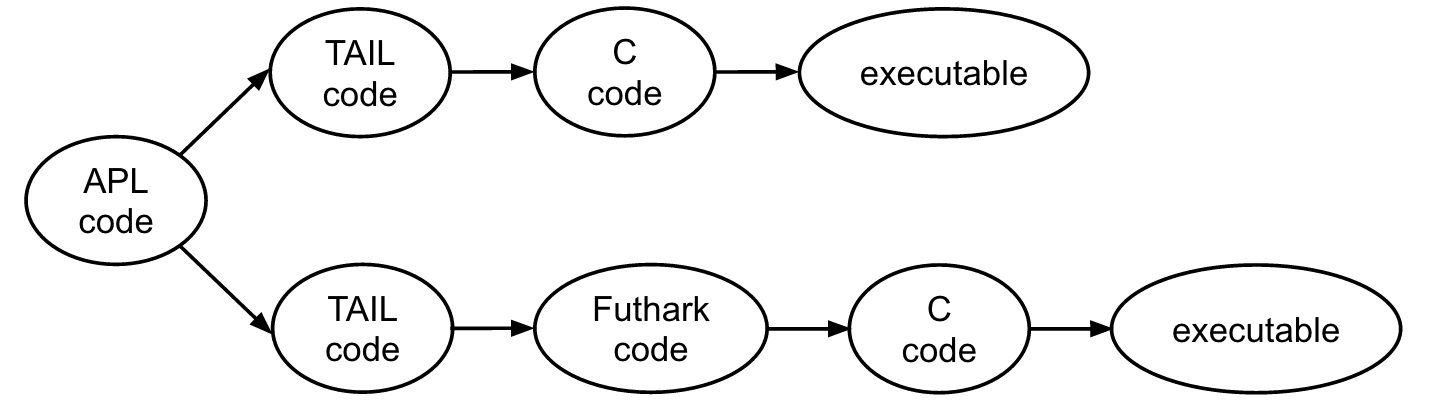
\includegraphics[width=11cm]{code.png}
    \caption{The path for a benchmark from APL to an executable file.}
\end{center}
\label{fig:code}
\end{figure}

Because no parallel backend was finished for either TAIL or Futhark when we did the benchmarks we use a sequential backend for both languages. 
The C-code is then compiled using a C compiler and the comandline tool {\tt time} is used to mesure the execution time. Each benchmark is run 10 times each and then the average is reported. The benchmarks and the results of the benchmarks are listed in Table 1.
The benchmarks is run on a Intel(R) Core(TM) i7-4500U CPU @ 1.80GHz. 

We made a Makefile to manage the building of the benchmarks. The Makefile is also placed in the {\tt tests/benchmarks} directory.


\subsection{Matrix multiplication}
The matrix multiplication benchmark takes a matrix and multiplies it with itself transposed.
It then reduces the resulting matrix twice, once by using times and once by using plus (times is used on the outer dimension).
The multiplication is done using reshape and then the arguments is transposed so they can be zipped with plus.
The impementation is in the file {\tt matmul.apl}

\subsection{Pi}
The pi benchmark approximates pi by computing the ratio of points in the range $[0,1] \times [0,1]$ that have a distance to $(0,0)$ of less than 1.
It does so by using $n \times n$ evenly spaced points in the interval $[0,1] \times [0,1]$, it can be helpful to imagine the set of points as a regular grid.
The more fine grained the grid the closer he approximation to pi.

The program first generates $n$ evenly spaced points in the interval $[0,1]$, it then squares those points before replicating them $n$ times to a $n \times n$ matrix.
Then the matrix is added with it's own transpose and from the resulting matrix is produced a boolean matrix
where all the entries with points with distance less than one from 0 are set to 1 and the rest to 0. Is is not necessary to take
the square root of the sums since that square root will be less that 1 only if the original sum is less that 1.
Finally the matrix is reduced with plus two times to get the number of points, the amount is divided by the total number of points and
this number is multiplied by 4 to get pi.
The impementation is in the file {\tt pi.apl}

\subsection{Black-scholes}
The black-scholes benchmark is taken directly from the bechmark suite of the APLTAIL compiler repository and computes the price of european style options. We have not modified this benchamark and while it doesn't give any insight into performance it demonstrates
that it is possible to compile this benchmark. 
The impementation is in the file {\tt blackscholes.apl}

\subsection{Easter}
The easter benchmark computes the date of easter and is found in the apltail project as {\tt tests/easter3000.apl}, the only
modification we have done is to make the date the result from the program instead of printing it and changed a parameter to scale
the program up.

The impementation is in the file {\tt easter3000.apl}

\subsection{Primes}
The primes benchmark computes the number of primes below $n$ and is found in the apltail project as {\tt tests/primes0.apl}.
Again we have only made the program return the result instead of printing it and scaled up the parameter $n$.
The APL program can be seen below:\\
\fbox{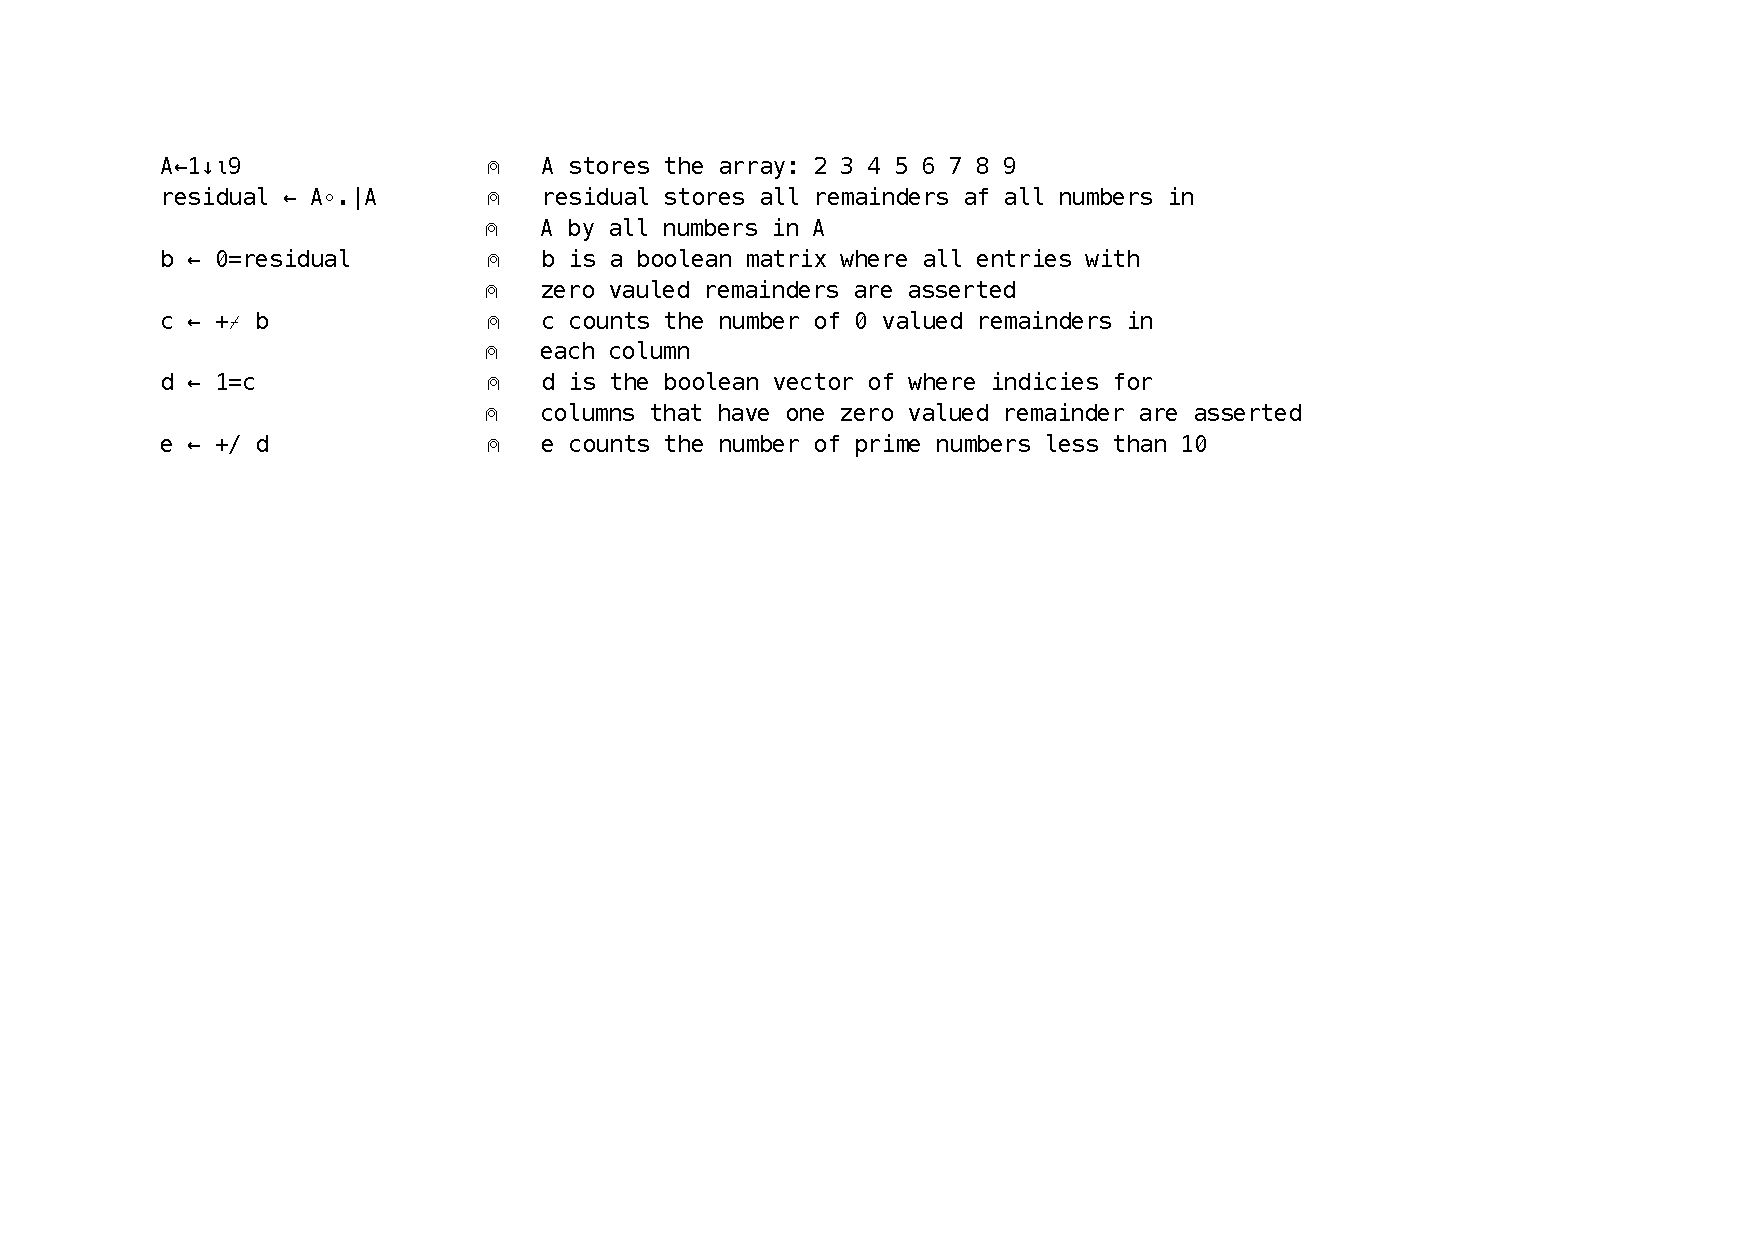
\includegraphics[scale=0.7,trim=6em 40em 10em 6em,clip=true]{primes.pdf}}
The APLTAIL compiler compiles the code to the following TAIL program:
\begin{lstlisting}[breaklines=true,language=TAIL]
let v1:<int>8 = dropV{[int],[8]}(1,iotaV(9)) in
let v7:[int]2 = transp{[int],[2]}(reshape{[int],[1,2]}([8,8],v1)) in
let v8:[int]2 = reshape{[int],[1,2]}([8,8],v1) in
let v11:[int]2 = zipWith{[int,int,int],[2]}(resi,v7,v8) in
let v18:[int]1 = transp{[int],[1]}(reduce{[int],[1]}(addi,0,each{[bool,int],[2]}(b2i,transp{[bool],[2]}(v13)))) in
let v13:[bool]2 = each{[int,bool],[2]}(fn v12:[int]0 => eqi(0,v12),v11) in
let v20:[bool]1 = each{[int,bool],[1]}(fn v19:[int]0 => eqi(1,v19),v18) in
let v24:[int]0 = reduce{[int],[0]}(addi,0,each{[bool,int],[1]}(b2i,v20)) in
i2d(v24)
\end{lstlisting}
The tail2futhark compiler then produces this result where the library functions are omitted:
\begin{lstlisting}[language=Futhark,breaklines=true]
fun real main() =
  let t_v1 = drop1_int(1,map(fn int (int x) => (x + 1),iota(9))) in
  let t_v7 = rearrange((1,0),reshape((8,8),reshape1_int((8 * (8 * 1)),reshape(((size(0,t_v1) * 1)),t_v1)))) in
  let t_v8 = reshape((8,8),reshape1_int((8 * (8 * 1)),reshape(((size(0,t_v1) * 1)),t_v1))) in
  let t_v11 = map(fn [int] ([int] x,[int] y) => map(resi,zip(x,y)),zip(t_v7,t_v8)) in
  let t_v13 = map(fn [bool] ([int] x) => map(fn bool (int t_v12) => (0 == t_v12),x),t_v11) in
  let t_v18 = rearrange((0),map(fn int ([int] x) => reduce(+,0,x),map(fn [int] ([bool] x) => map(boolToInt,x),rearrange((1,0),t_v13)))) in
  let t_v20 = map(fn bool (int t_v19) => (1 == t_v19),t_v18) in
  let t_v24 = reduce(+,0,map(boolToInt,t_v20)) in
  toFloat(t_v24)
\end{lstlisting}

% For at vise et større eksempel har vi medtaget det her benchmark
% Man kan se parallel operatorer bliver oversat til andre parallele operatorer
% Man kan se transformation af curried lambdaer
% Biblioteksfunktioner bliver brugt

The impementation can also be seen in the file {\tt primes0.apl}\\
\subsection{Results}

In all of the benchmarks except black-scholes we have seen significant speed-ups by compiling to Futhark.
The biggest difference was in the pi benchmark, this is due to the fact that the APLTAIL compiler ends up fusing too much and
duplicates work. It calculates $x * x$ $n^2$ times instead of just $n$ times as expressed in the APL program.
This is a limitation the authors are aware of and describe in their publication \cite{Array:2015}.
It remains to be seen whether these results are reproducible on parallel hardware.

\section{Discussion}
\label{sec:discussion}
In this section we discuss the viability of the approch we have used, what we have learned in the project and ideas for future work. 

Our main goal has been to see if it is possible, effectively to compile TAIL programs, into Futhark programs and thereby make use of the Futhark infrastructure for optimisation and the possibility for targeting parallel hardware.

We have been able to compile TAIL to Futhark code using parallel constructs in Futhark whenever we encountered parallel constructs in TAIL.
Because of this we have reason to believe that no parallelism has been eliminated during the compilation.
Although we have not veriefied the effect the compilation has on performance on parallel hardware we have seen significant speed-ups
in sequential execution as measured in our benchmarks and are confident that these speed-ups can be reproduced on parallel hardware.
We feel these sequentially executed benchmarks are relevant because the are parallel in their structure and should therefore execute efficiently on parallel
 hardware.
 
 % dataparallelisme, hvile ting er forskellige er vigtige for dem, fx memory paa GPU. Tilgang paa 
 % stoerre forstaaelse for hvad der inpacter/har betydning for parallelisme

During this project we have learned the value of using a mathematical notation to work from and to present and reason about in the form of our compilation scheme. 
Without our compilation scheme it is not clear how to present the work, either we would have to argue based on the
implementation which muddles the picuture with implementation details, or we would have to argue in prose which
makes it difficult to precisely explain the concepts without being very verbose.
The notation is also a good tool for communicating during the development of the ideas for compilation, because it is programming language independent.

Also we have learned that the type systems means a lot when compiling between languages. 
In our concrete example we had an issue with polymorphism.
This made the compilation a lot less simple since we had to make design desisions on how to handle this in the best way and what the best way was. 
We decided to create library functions for each basic type and create our compilation so that we only used library functions in the one-dimensional case.
Otherwise we could have made a function for each version of basic type and array shape for a limited set of combinations. But this means we could not have supported a significant portion of TAIL.


If we had to redo this project we would have focused more on the benchnarks from the beginning as soon as we
started implementing. This makes for a more goal oriented work-flow instead of the check-list like work-flow we had.
Maybe we would have implement fewer operators and instead focus on analyzing the code generated by the compilers (APLTAIL and Futhark) and
from that argue about the soundness of our conversion rules.

As we began our project no parallel backends for either languages were available, however towards the end of the project a
parallel backend for TAIL using Accelerate had been published \cite{Array:2015} and a parralel backend for Futhark using OpenCL
was in development.

It would be interesting to test the bechmarks with the parallel backends to compare TAIL and Futhark on parallel hardware.
Depending on the results it could be interesting to look at the generated C code to see the cause of the differences in the
runtime of the benchmarks.

Finaly, it could also be interesting to try out bigger and more comprehensive benchmarks and compare the runtimes.

\section{Conclusion}
\label{sec:conclusion}

 % forklar kort hvad der var i rapporten
% Hvad var det vi ville i forhold til projektet/ hvad var vores tese
% Svar paa om vi har opnaaet det. 

In this paper we have desribed relevant part of the two languages TAIL and Futhark. 
We have also presented a compilation between the two languages shown in an implementation independent mathematical notation as well as an implementation of this scheme in Haskell and test of this implementation. 
Finaly, we have compaired the execution time of selected benchmarks. 

In this project we wanted to examine if it was possible, effectively to compile TAIL programs, into Futhark programs and thereby make use of the Futhark infrastructure for optimisation and the possibility for targeting parallel hardware.

We have shown that it is possible to effectivly compile TAIL to Futhark by expressing this compilation in a compilation scheme done in a mathematical notation that is language independent and also implement this compilation scheme in Haskell. We have used the Haskell implementation to test the correctness of the compilation scheme. 
We have preserved the parallelism in the code by ensuring that all parallel operators in TAIL are mapped to parallel functions in Futhark. 
Compiling the code with the Futhark compiler has the benefit of optimizing the code as we have measured significant speed-ups from utilizing the Futhark compiler in our benchmarks.


%%%%% references %%%%%
\bibliography{references}{} 
\bibliographystyle{plain}

\newpage

\appendix
\section{Parser source code}
\label{app:parser}

In this appendix is the source code for the APLACC parser \cite{APLACC} with the motifications we added.
We did not develop the code presentet in this appendix but only made small alterations to the existing code. A describtion of the alterations we did add can be found in Section \ref{sec:parser} and can also be seen in the commits in the github repository for our project. 

\lstset{breaklines=true}

\lstinputlisting[language=haskell,  mathescape=false]{../aplacc/src/APLAcc/TAIL/Parser.hs}

\newpage

\section{Compiler source code}
\label{app:impl}

This appendix contains the source code of the TAIL2Futhark compiler found in file {\tt src/Tail2Futhark/Compile.hs}. 
\lstinputlisting[language=haskell,  mathescape=false]{../src/Tail2Futhark/Compile.hs}

\newpage

\section{Pretty printer source code}
\label{app:pretty}

This appendix contains the source code of the pretty printer used to print the Futhark AST. The pretty printer are located on the following path in the project: {\tt src/Tail2Futhark/Futhark/Pretty.hs}. 

\lstinputlisting[language=haskell,  mathescape=false]{../src/Tail2Futhark/Futhark/Pretty.hs}

\newpage

\section{Test results}
\label{app:testresults}
The tests can be found in the {\tt test/basic\_tests/} directory in our project.
The expected result of the test can be found in the .ok version of the file. The results in the table below is OK if the result of the compilation (found in the .out file) matches the expected one or FAIL if it does not.

\begin{center}
\begin{tabular}{l l l l}
Function  		& File name		& Describtion of test			& Result \\ \hline \\
negi			& negi.tail			& negtes ints				& OK \\
negd 		& negd.tail			& negate double				& OK \\
ln 			& blacksholes.tail	& -					& blacksholes evaluates to correct result \\
absi 			& blacksholes.tail	& -					& blacksholes evaluates to correct result \\
expd 		& blacksholes.tail	& -					& blacksholes evaluates to correct result \\
mini 			& mini.tail			& min on 2 positive ints		& OK \\
signd 		& signd.tail			& sign of double				& OK \\
notb			& not1.tail			& not on true				& OK \\
notb			& not0.tail			& not on false				& OK \\
maxi			& maxi.tail			& max on 2 positive ints		& OK \\
maxd		& maxd.tail		& max on 2 positive doubles	& OK \\
ori			& 				& NOT TESTET				&  \\
subi			& subi.tail			& substract positive ints		& OK \\
subd			& subd.tail			& substract positive doubles	& OK \\
muli			& muli.tail			& multiply 2 positive ints		& OK \\
muld			& muld.tail			& multiply 2 positive doubles	& OK \\
ltei			& ltei.tail			& 4 $\leq$ 3				& OK \\
ltei			& lteiTrue.tail		& 4 $\leq$ 5				& OK \\
lted			& lted.tail			& 2.3 $\geq$ 3.3				& OK \\
eqi			& eqiTrue.tail		& 4 $=$ 4					& OK \\
eqi 			& eqiFalse.tail		& 4 $=$ 5					& OK \\
eqd			& eqdFalse.tail		& 3.4 $=$ 1.2				& OK \\
gti			& gtiTrue.apl		& 5 $>$ 4					& OK \\
gtd			& gtdTrue.apl		& 3.4 $>$ 1.2				& OK \\
gtei			& gteiTrue.tail		& 3 $\geq$ 2				& OK \\
gted			& gtedFalse.tail		& 3.0 $\geq$ 3.2				& OK \\
andb 		& andbTrue.tail 		& (2 $=$ 2) $\land$ (3 $=$ 3)	& OK \\
orb			& orFalse.tail		& (2 $=$ 1) $\lor$ (3 $=$ 2)		& OK \\
orb			& orTrue.tail		& (2 $=$ 1) $\lor$ (2 $=$ 2)		& OK \\
divi 			& divi.tail			& (4 / 2) + 4				& OK \\
divd			& divd.tail			& (4.0 / 2.0) + 4				& OK \\
powd			& powd.tail			&  FORKERT tester ints		&  \\
powi			& powi.tail			& power on 2 positive ints		& OK \\
lti			& ltiTrue.tail 		& 3 $<$ 5					& OK \\
ltd			& ltdTrue.tail 		& 3.2 $<$ 5.1					& OK \\
andi			& - 				& 				          	& \\
xorb			&  xorb.tail 		& (3=3) $\neq$ (4=1)				& OK \\
i2d 			& i2d.tail			& integer to double 			& OK \\
addi 			& addi.tail 			& addition of 2 positive ints		& OK \\ 
addd 		& addd.tail 		& 2.3 + 4.5					& OK \\
iotaV 		& iotaV.tail			& iota in positive integer		& OK \\
iota	 		& iotaV.tail			& iota in positive integer		& OK \\
eachV		& eachV.tail  		& add int on vector of ints 		& OK \\
each			& each.tail			& add int on matrix af ints 		& OK \\
reduceV		& - 				&						&  \\
reduce		& reduceRank0.tail	& reduce on vektor of int		& OK \\
reduce 		& reduce2.tail		& reduce on matrix of int		& OK \\
reduce 		& reduce3.tail		& reduce on array of rank 3 	& OK \\	
shapeV		& firstV2.tail		& shape of vector			& OK \\
shape		& take2.tail		& shape of matrix of ints		& OK \\
\end{tabular}
\end{center}

\begin{center}
\begin{tabular}{l l l l}
Function  		& File name		& Describtion of test						& Result \\ \hline \\
reshape		&  reshape.tail		& reshapes vector of int with padding			& OK \\
reshape 		& reshape2.tail	 	& reshape vector into array of rank 			& OK \\ 
vreverse		& rev2.tail			& reverse of matrix of ints					& OK \\
vreverseV		& rev.tail			& reverse of vector of ints					& OK \\
vrotate		& rotateRank2.tail	& rotate array of rank 3 of ints				& OK \\
vrotateV		& rotateRank1.tail	& rotate vektoof ints 						& OK \\
transp		& transp2.tail		& transpose vector of ints					& OK \\
transp 		& transp3.tail		& transpose array of rank 3 of ints			& OK \\ 
transp 		& transpAPL.tail		& transpose matrix of ints					& OK \\	
transp2		& dyadic\_transp.tail	& transpose of matrix of ints				& OK \\
takeV		& take1.tail		& positive int on vector with enough elements 	& OK \\ 
takeV		& take1neg.tail		& negative int on vector with enough elements	& OK \\ 
take			& take2.tail		& positive int on matrix with enough elements 	& OK \\
dropV		& drop2.tail		& positive int on vector with enough elements	& OK \\
drop			& drop2Dim.tail	    	& drops row in array rank 2 with enough elements & OK \\
drop 			& drop2DimNeg.tail 	& drops with a negative number on array of rank 2 & OK \\
drop 			& drop2DimtoMuch.tail & drops more rows than there are in the array     & OK \\
drop 			& drop3Dim.tail		& positive int in a 3 dim array				& OK \\ 
consV		& -				&									&  \\
cons			& cons1.tail		& vector of ints on array of rank 2 of ints		& OK \\ 
snocV		& snocRank1.tail 	& set scalar on vector						& OK \\
snoc			& snocRank2.tail	& set vector on matrix 					& OK \\
firstV			& firstV2.tail		& first element of vektor with only one element	& OK \\
firstV			& firstV3.tail 		& first element of vektor of ints				& OK \\
first			& first2.tail			& first on a matrix						& OK \\
zipWith		& zipwith.tail		& zip addi over two vectors					& OK \\ 
zipWith 		& zipwith2.tail		& zip addi over two matrices				& OK \\
zipWith 		& zipwith3.tail		& zip addi over two arrays of rank 3 of ints		& OK \\
catV			& - 				& 									& \\
cat			& cat.tail			& cat of arrays of rank 2 of ints				& OK \\
cat			& catV.tail			& cat of vectors of ints					& OK \\
cat			& concat.tail		& cat of arrays of rank 2 af ints				& OK \\
reshape		& reshape.tail		& reshape vector to matrix					&  OK \\
reshape		& reshape2.tail		& reshape with extending the vector			&  OK \\
\end{tabular}
\end{center}

\end{document}
